% Document layout
\documentclass[a4paper,11pt]{article}
\usepackage[a4paper, inner=2.5cm , outer=2.5cm, top=2cm, bottom=2cm]{geometry}
\usepackage[usenames,dvipsnames]{color}
% Referencing & fonts
\usepackage[sort&compress]{natbib}
\setlength{\bibsep}{0.0pt}
\usepackage[font=small,labelfont=bf]{caption}
\usepackage[OT2,T1]{fontenc}
% Set formats for each heading level
\usepackage{sectsty}
\allsectionsfont{\usefont{OT1}{phv}{bc}{n}\selectfont}
\sectionfont{\color{MidnightBlue}} % sets colour of sections
\subsectionfont{\color{MidnightBlue}}  % sets colour of subsections
\subsubsectionfont{\color{MidnightBlue}}  % sets colour of subsections
% Other shit
\usepackage{algorithm}
\usepackage{amsfonts}
\usepackage{amsmath}
\usepackage{amssymb}
\usepackage{bbm}
\usepackage{booktabs}
\usepackage{epsfig}
\usepackage{float}
\usepackage[font=normalsize]{caption}
\usepackage{graphicx}
\usepackage{hyperref}
\usepackage{lineno}
\usepackage{mathtools}
\usepackage{sidecap}
\usepackage{sectsty}
\usepackage{verbatim}
\usepackage{wrapfig}
\usepackage{xcolor}
\usepackage{listings}
\lstset{
  basicstyle=\small\ttfamily,
  columns=flexible,
%  numbers=left,
  breaklines=true
  }
% Declarations
\DeclarePairedDelimiter\floor{\lfloor}{\rfloor}
\DeclareSymbolFont{cyrletters}{OT2}{wncyr}{m}{n}
\DeclareMathSymbol{\Sha}{\mathalpha}{cyrletters}{"58}
\DeclareMathSymbol{\sha}{\mathalpha}{cyrletters}{"57}
% Defined commands
 \newcommand{\prgname}[1]{\textcolor{NavyBlue}{\texttt{#1}}}
 \newcommand{\linkfont}[1]{\textcolor{BurntOrange}{\textbf{#1}}}
\newcommand{\shellcmd}[1]{\\\indent\indent\texttt{\$ #1}}
\newcommand{\shellctd}[1]{\\\indent\indent\texttt{#1}}
\newcommand{\ra}[1]{\renewcommand{\arraystretch}{#1}}
\begin{document}
\begin{figure}
\centering
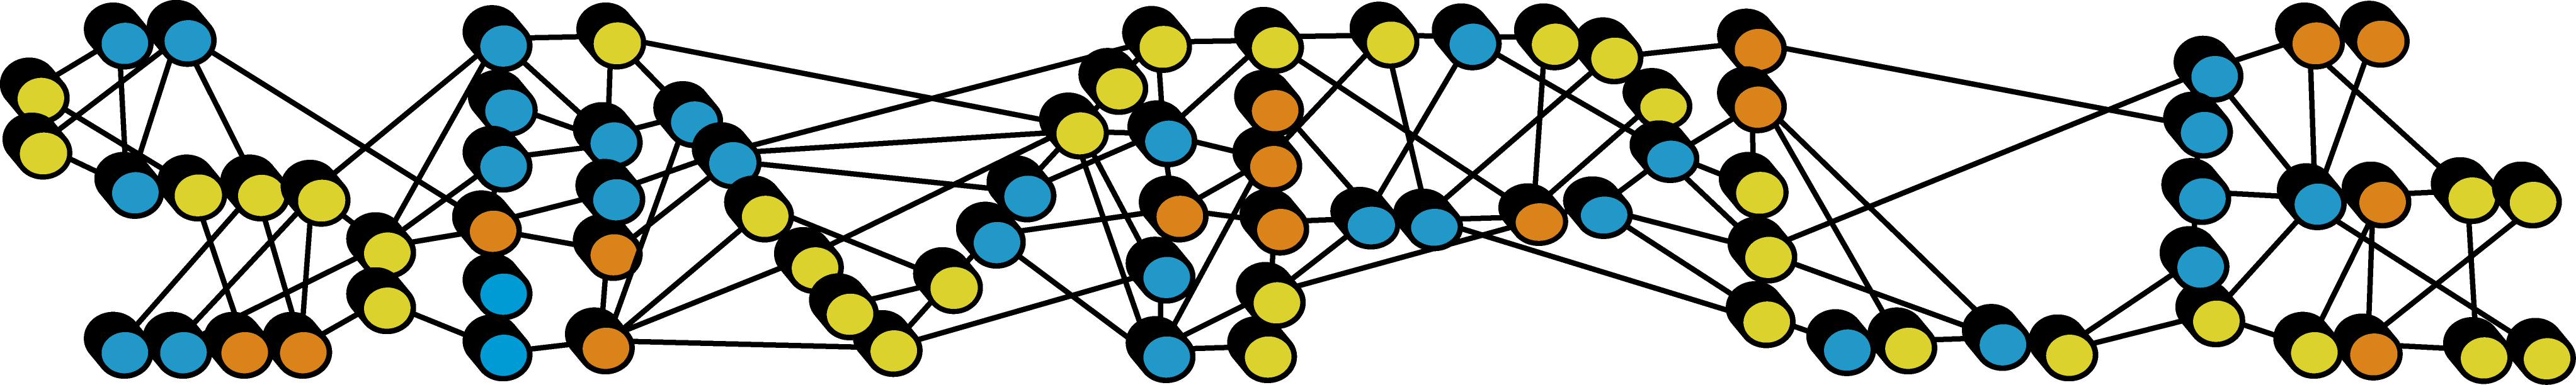
\includegraphics[keepaspectratio=true,scale=0.6]{./SIMPLE_logo/rawlogo}
%\caption{}
\end{figure}

\title{\prgname{Developers Guide to SIMPLE}}
\date{Christmas Day, 2016}
\author{Hans Elmlund}
\maketitle

\vspace{1em}
\begin{minipage}[ht]{0.48\textwidth}
\textbf{Contributors:}\\
cyril.reboul@monash.edu\\
michael.eager@monash.edu\\
dominika.elmlund@monash.edu\\
hans.elmlund@monash.edu\\
\textbf{Adress:}\\
Dept. Biochemistry and Molecular Biology\\
School of Biomedical Sciences\\
Monash University, Bldg. 77\\
Clayton, VIC, Australia, 3800\\
\textbf{Webpage:}\\
www.simplecryoem.com\\
\end{minipage}
\vspace{20pt}

\begin{quote}
\textbf{``Keep it SIMPLE stupid''}\\(\textit{Kelly Johnson}; lead engineer at the Lockheed Skunk Works, coined the famous KISS principle stating that systems work best if they are kept simple rather than made complex. Therefore, simplicity should be a key goal in design and unnecessary complexity should be avoided.)
\end{quote}

\begin{quote}
\textbf{``Everything should be made as SIMPLE as possible, but no SIMPLEr''}\\(\textit{Albert Einstein})
\end{quote}

\begin{quote}
\textbf{``Complex theories do not work, SIMPLE algorithms do''}\\(\textit{Vladimir N. Vapnik}; author of \textit{The Nature of Statistical Learning Theory})
\end{quote}
\clearpage

\tableofcontents{}
\clearpage

\section{Disclaimer}
Many of the general ideas/concepts presented in this document are not my original contributions but direct or modified rip-offs from other people's work, including Eric Evans' ``Domain-Driven Design, Tackling Complexity in the heart of Software'', the gang of four's classic work ``Design Patterns: Elements of Reusable Object-Oriented Software'', Damian Rouson's ``Scientific Software Design: The Object-oriented Way'' in addition to a number of Fortran language reference books. This document is therefore not intended for distribution but will serve as a guide for those developing code (or improving the model behind the code) within the SIMPLE environment.

\section{A Domain Model for SIMPLE Development}

\subsection{The Two Most Important Design Principles}
Before we start the esoteric discussion about object-oriented design philosophy, let's keep it simple. There are two principles of software design that have been repeated so many times in development documents and programming books that their origins are long forgotten. These are the two most important design principles, whether you are working on a fancy object-oriented library, hacking in procedural C code, writing a jiffy perl script or creating assembly code for a driver.
\begin{enumerate}
\item \textbf{DRY:} \textbf{D}on't \textbf{R}epeat \textbf{Y}ourself. No matter how convenient it is to cut and paste snippets of code and introduce some slight modifications when your head is buzzing with ideas and you want to test something NOW there is NEVER any justification for duplicating code. Repetitions are costly, they force you to update the same logics in multiple places in the library and it makes debugging a living hell. \textbf{DRY!!!}
\item \textbf{YAGNI:} \textbf{Y}ou \textbf{A}in't \textbf{G}onna \textbf{N}eed \textbf{I}t. A lot of time has been wasted in the name of completeness. Even if your clever maths routine can be tuned into accepting arrays of any shape or type, if the need that you have RIGHT NOW is for it to operate on real one-dimensional arrays, then only code the routine for the real one-dimensional arrays. Because chances are, if you extend it to all conceivable cases: \textbf{Y}ou \textbf{A}in't \textbf{G}onna \textbf{N}eed \textbf{I}t! And you end up with a lot of dead code in the library that those that come in as new developers will have to plow through and try to understand, only to realise they just wasted their time. Dead code should preferably never be written but if sections are dying as development progresses, better move them to a legacy folder of some sort.
\end{enumerate}

\subsection{One Team, One Language}
It is the nature of software to change, and SIMPLE has continued to evolve in the hands of the team that owns it. This document arouse because of the need for guiding design principles to keep the growing team focused and productive. SIMPLE is written in modern Fortran. It is crucial that every SIMPLE developer masters object-oriented Fortran 2008 programming. The core functionality of SIMPLE is accomplished by a set of layered classes that meet in modules that define their functional relationships and data sharing interconnections. Although these modules represent high-level abstractions that drive a lot of the functionality of the library, there are additional layers that serve to allow the simultaneous design of high-level workflows (user-oriented) and finely chopped functionality (expert-oriented) required for proper testing and effective development. Before we dig into the details of it all, I will describe the overall development and design philosophy of SIMPLE. The principles and guidelines outlined here are not necessarily implemented in the current version of SIMPLE but with common efforts and ruthless refactoring I believe we will get there.

The phrase \textit{One Team, One Language} comes from Eric Evans' book on domain-driven design and has nothing to do with the programming language used. Instead, \textbf{it refers to the concept of \textit{ubiquitous language}. With a \textit{ubiquitous language}, conversations among developers, discussions among domain experts, and expressions in the code itself are all based on the same language, derived from a shared domain model.} Our domain model represents the steps required to process electron microscopy images of particles (biological as well as inorganic nanoparticles). The model should support analysis of particles of any symmetry (helical or point-group), accept images from any kind of microscope (200kV, 300kV, with or without phase-plate etc.) or electron detector, and be applicable to 2D (single-particle) and 3D (subtomographic averaging) particles alike. Currently, the support for tomography is weak (limited to motion-correction and dose-weighting of tomographic tilt-series) and substantial additional coding and refactoring of existing library parts will be required to support analysis of subtomograms with already established correlation/search/CTF methods. The model should furthermore support efficient parallel execution of SIMPLE on heterogeneous clusters and workstations, including hybrid CPU/GPU architectures, in a user-friendly manner.

\subsection{Modelling the Domain: Why Bother?}
If the coders don't feel responsible for the model, or don't understand how to make the theory underpinning the model work for an application, the model has nothing to do with the software. If developers don't realise that changing the code changes the model, then their refactoring will weaken the model rather than strengthening it. When a modeler is separated from the implementation process, he or she never acquires or quickly loses, a feel for the constraints of the implementation. \textbf{The basic constraint of \textit{model-driven design} is that the model supports an effective implementation and abstracts key domain knowledge. The knowledge and skills of experienced designers will  be transferred to other developers if the division of labour allows the kind of collaboration that conveys the subtleties of coding a \textit{model-driven design}.} Currently, the two most experienced model-driven SIMPLE coders are Cyril and Hans. The reason for this is that we have invested 50/50 into the model (I want to solve an accurate \textit{ab initio} structure with EM) and the code that expresses the model. When additional collaborators/coders enter the team, it is important that we explain the principles even though we cannot expect that everyone will invest equally into the model and the code. For example, Dominika is 100\% model at the moment but I do anticipate that Alex will start contributing to the code base and the scientific programmer that we will employ will have to focus a large part of his/her initial efforts into understanding the model. Anyone responsible for changing code must learn to express the model through the code. Every developer must be involved in some level of discussion about the model and have regular contact with domain experts (many of which are our users). Those who contribute in different ways must consciously engage those who touch the code in a dynamic exchange of model ideas through the \textit{ubiquitous language}.

\subsection{The Layered SIMPLE Architecture}
Partition a complex program into layers. Develop a design within each layer that is cohesive and that depends only on the layers below. Follow standard architectural patterns to provide loose coupling to the layers above. Concentrate all the code related to the domain model in one layer and isolate it from the user interface, application and infrastructure code. The domain objects, free of the responsibility of displaying themselves, storing themselves, managing application tasks, and so forth, can be focused on expressing the domain model. This allows a model to evolve to be rich enough and clear enough to capture essential research knowledge and put it into work. SIMPLE was designed in a layered fashion.
\begin{SCfigure}[][h]
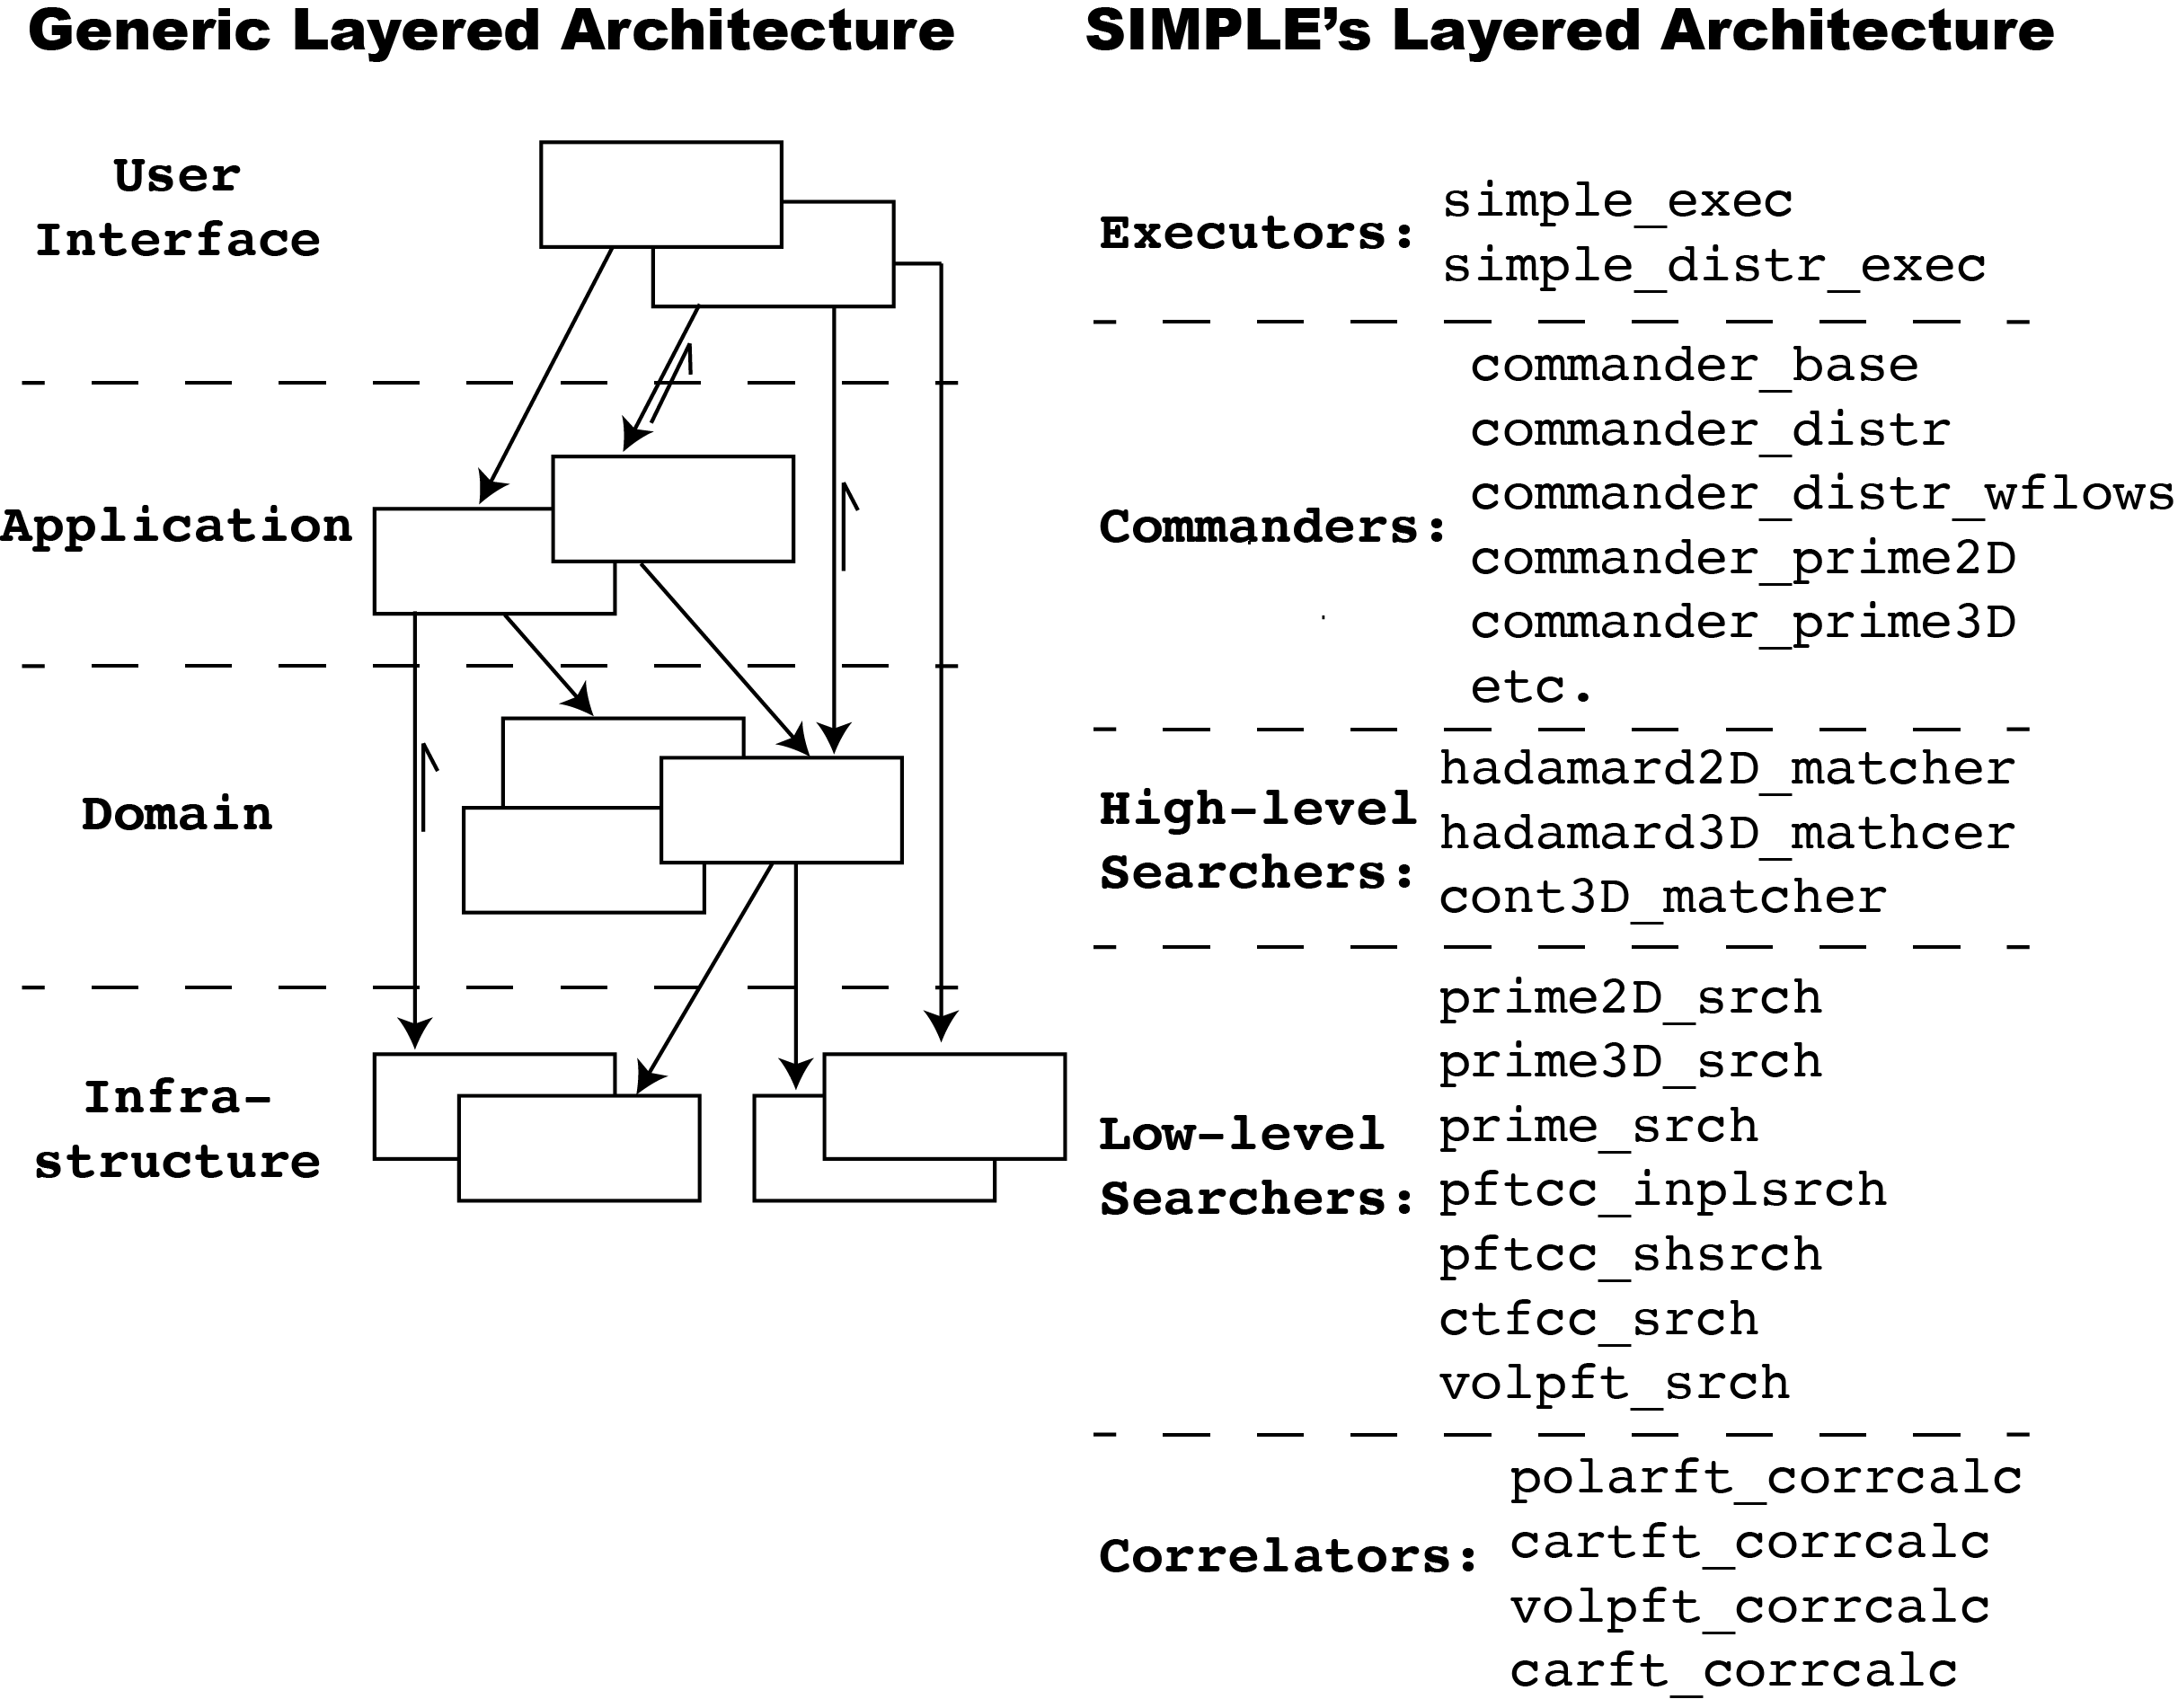
\includegraphics[keepaspectratio=true,scale=0.6]{./LayeredArch/layered_arch}
\end{SCfigure}

Layering the design was not something that we really thought long and hard about. The layered structure evolved as a natural consequence of creating units that express fundamental components of the domain model. At the root level are the correlators that evaluate the goal function (correlation) in different settings.
\begin{verbatim}
simple_cartft_corrcalc.f90   ! calculates correlations between 2D Cartesian FTs
simple_comlin_corr.f90       ! calculates common line correlations
simple_polarft_corrcalc.f90  ! calculates correlations between 2D polar FTs 
simple_volpft_corrcalc.f90   ! calculates correlation between volume FTs
\end{verbatim}
These classes have very few dependencies, the most notable one being the builder. These are the number crunchers of the SIMPLE library. About 60\% of the computations in the the PRIME2D/3D searches consists of calculating correlations. It is in this area we will focus our efforts in performance enhancement by designing data structures that make efficient use of cache and data structures that scale up the matrix sizes so that the calculations can be efficiently done on GPUs. In the next level up are the low-level searchers.
\begin{verbatim}
simple_cftcc_srch.f90     ! continuous search using cartesian FTs
simple_comlin_srch.f90    ! basic common lines search routines
simple_comlin_symsrch.f90 ! symmetry search routines
simple_ft_shsrch.f90      ! origin shift search for Cartesian FTs
simple_ftexp_shsrch.f90   ! fast origin shift search using expanded Cartesian FTs
simple_pftcc_inplsrch.f90 ! discrete/continuous in-plane parameter polar FT search
simple_pftcc_shsrch.f90   ! origin shift search for polar FTs
simple_prime2D_srch.f90   ! search routines used in PRIME2D
simple_prime3D_srch.f90   ! search routines used in PRIME3D
simple_prime_srch.f90     ! search routines common to PRIME2D/3D
simple_symsrcher.f90      ! symmetry axis search routines
simple_volpft_srch.f90    ! volume registration search routines
\end{verbatim}
The most prominent role of these classes is to put together the correlators with the classes responsible for the optimisation. The most important classes in this group are the \texttt{prime2D\_srch} and \texttt{prime3D\_srch} classes who shares common functionality via the \texttt{prime\_srch} class. In order to understand the algorithmic details of the stochastic optimisation implemented in the PRIME algorithm, look in the \texttt{prime2D\_srch} and \texttt{prime3D\_srch} classes. In the next level we find the modules executing the projection-matching-based algorithms.
\begin{verbatim}
simple_cont3D_matcher.f90      ! continuous projection matching
simple_hadamard2D_matcher.f90  ! discrete 2D clustering and alignment
simple_hadamard3D_matcher.f90  ! discrete 3D ab initio reconstruction
\end{verbatim}
Most designs would now have ended with a final layer of executables with an associated user interface. However, in SIMPLE we use a trick based on a design pattern called \textit{commander} (described below) to ``objectify'' the execution of a program. This means that the concept of ``executing PRIME2D'' is encapsulated in a class that can be instantiated to create objects. The commander classes have only a single method ``execute''. Why bother complicating things in this manner? Because now we can create arrays of executables and we can systematically vary the input parameters and make a computer program that automatically does this for us. This, of course, has fundamental implications for the design of unit tests or restart methodologies. It also makes it possible to create high level workflows that combine virtually every functionality of the library. Moreover, it lends itself readily to highly efficient job scheduling in cluster environments and on workstations. By studying the commander classes in SIMPLE we get a feel for the high-level functionalities and how they can be combined to create advanced and highly automated workflows.
\begin{verbatim}
simple_commander_base.f90          ! the abstract base class
simple_commander_checks.f90        ! simple check commanders
simple_commander_comlin.f90        ! common lines commanders
simple_commander_distr.f90         ! commanders used in distributed execution
simple_commander_distr_wflows.f90  ! the parallel high-level workflows
simple_commander_imgproc.f90       ! basic image processing commanders
simple_commander_mask.f90          ! masking commanders
simple_commander_misc.f90          ! miscellaneous commanders
simple_commander_oris.f90          ! orientation commanders
simple_commander_preproc.f90       ! pre-processing commanders
simple_commander_prime2D.f90       ! prime2D commanders
simple_commander_prime3D.f90       ! prime3D commanders
simple_commander_rec.f90           ! volume reconstruction commanders
simple_commander_sim.f90           ! simulation commanders
simple_commander_volops.f90        ! miscellaneous volume operation commanders
\end{verbatim}
Lastly, we have the executable layer.
\begin{verbatim}
simple_exec       ! shared-memory parallelisation mode
simple_distr_exec ! hybrid distributed/shared-memory parallelisation mode 
\end{verbatim}
The distinction between these two execution routes will be explained in detail below.

\section{The Building Blocks of SIMPLE}

\subsection{SIMPLE Classes}

\subsubsection{Classes are a Special Kind of Modules}
Fortran has three main design elements: subroutines, functions and modules. Fortran does not have a specific element implementing a class but uses the module construct  to make classes that instantiate objects.
\begin{verbatim}
!==Class simple_example
!
! simple_example is just a dummy example for how to implement a generic class
!
module simple_example
use simple_defs                           ! module with parameters
use simple_other_class, only: other_class ! type(other_class)
implicit none                             ! no implicit variable declaration

! we only make the instance and the unit test public; everything else is private
public :: example, test_example 
private                         

! class parameter
integer, parameter :: my_class_variable=10

! the abstract data type (instance definition)
type example
    private                                      ! data encapsulation
    type(other_class) :: my_other_class_instance ! this is composition
    real, allocatable :: my_real_arr(:)          ! allocatable array declaration
    logical           :: exists = .false.        ! to indicate existence
contains                                         ! after contains comes the methods
    procedure :: new                             ! conventional name of constructor
    procedure, private :: method1                ! this is generic programming
    procedure, private :: method2                ! within the class
    generic :: method => method1, method2 
    procedure :: kill                            ! conventional name of destructor
end type example

interface example
    module procedure constructor
end interface example

! after the contains statement comes the implementation of the methods
contains
\end{verbatim}
The first statements after the \texttt{module} statement are the \texttt{use} statements. Only modules that are required by most methods in the class should be declared here, otherwise we put them with the relevant methods (subroutines/function after last contains statement). Also, classes that are components of the example class need to be declared here. Inheritance by composition is almost always preferable to inheritance by type extension, but later we will look at examples where inheritance between abstract base classes and concrete implementing classes provides powerful means for run-time polymorphism. The following \texttt{implicit none} statement is a leftover from the olden days when Fortran used implicit variable declaration based on the first character of the variable name. Don't scatter implicit none statements all over the shop\textemdash{}it is sufficient to have them in the \texttt{program} units and in the top of the \texttt{module}. In SIMPLE, we use the convention that all code-containing files start with \texttt{simple\_} and if they are bona-fide classes, they are followed by the name of the abstract data type \texttt{simple\_example}. If they are modules rather than classes (we will come to this distinction later)  they are named according to the domain specific functionality that the module implements, for example \texttt{simple\_hadamard2D\_matcher}. Next, we declare class variables or parameters that are available throughout the scope of the module but inaccessible to the outside world. The abstract data type is declared just as an ordinary derived type with two exceptions:
\begin{enumerate}
\item The data is encapsulated (hidden to the outside world) via the \texttt{private} statement. This is one of the most important aspects of object-oriented programming. It allows the namespace of the abstract data type to be public in the instantiated object rather than the data itself. There are instances where it is practical to violate encapsulation, but we'll come to that later.
\item There's a \texttt{contains} section within the abstract data type that declares the names of the methods creating or in other ways operating on the data declared in the type. This is the mechanism whereby an instance of the example class carries the namespace of the methods. Methods are public by default (visible to the using unit) and made private (callable only within the scope of the module) via the \texttt{private} statement.
\end{enumerate}
\texttt{new} is the name convention we use for the constructor. We can do generic programming within the class for methods that are so closely related that they should have the same name, assuming that they have unique interfaces. \texttt{kill} is the name convention we use for the destructor. The  code snippet
\begin{verbatim}
interface example
    module procedure constructor
end interface example
\end{verbatim}
allows us to create instances in the using unit with the syntax
\begin{verbatim}
my_example_instance = example( <dummy arguments> )
\end{verbatim}
as we shall see shortly. Now to the implementation of the constructors:
\begin{verbatim}
...
interface example
    module procedure constructor
end interface example

! after the contains statement comes the implementation of the methods
contains

    subroutine new( self, other_specs, n )
        use simple_jiffys, only: alloc_err
        ! dummy variables are dealt with first
        class(example), intent(inout) :: self
        integer,        intent(in)    :: other_specs(:)
        integer,        intent(in)    :: n
        ! here comes the local variable declarations
        integer :: alloc_stat
        ! we always start with destructing a possibly pre-existing instance
        call self%kill
        ! construct the composite
        call self%my_other_class_instance%new(other_specs)
        ! allocate the array
        allocate( self%my_real_array(n), stat=alloc_stat)
        call alloc_err( "In: simple_example :: new", alloc_stat)
        ! indicate existence of the instance
        self%exists = .true.
    end subroutine new
\end{verbatim}
Methods in a class are implemented as standard subroutines or functions that have been part of the language specification since Fortran 77. We begin with declaring the units we need to use via \texttt{use simple\_jiffys, only: alloc\_err}. Even though the \texttt{simple\_jiffy} module contains a large number of subroutines and functions it is good programming practice to only declare exactly what is being used via the \texttt{only} directive. Following the use statements, we deal with the input dummy variables, which include the instance (named \texttt{self} by convention), the specification for creating the composite object \texttt{other\_specs} and the size of the array \texttt{n}. Note that we declare self as a polymoprhic variable by using \texttt{class} rather than \texttt{type} directive. The reason for this is that we may later use \textit{inheritance} for extending the example type, creating child classes that would need to use the example constructor.  The \texttt{intent} directive gives the intent of the dummy variables \texttt{in}, \texttt{out} or \texttt{inout} (see Fortran language reference). After input specification, we declare local variables. The execution section in a constructor always start with destructing the possibly pre-existing instance before proceeding with constructing the composite, allocating the array and indicating existence. Note that the symbol used to access the object's methods is \texttt{\%} in contrast to the \texttt{.} used in C++, Java, Ruby, Python and most other object-oriented languages. Often we also implement a function-based constructor:
\begin{verbatim}
...
interface example
    module procedure constructor
end interface example

! after the contains statement comes the implementation of the methods
contains

    function constructor( other_specs, n ) result( self )
        integer, intent(in) :: other_specs(:)
        integer, intent(in) :: n
        type(example)       :: self
        call sefl%new( other_specs, n )
    end function constructor

    subroutine new( self, other_specs, n )
        use simple_jiffys, only: alloc_err
        ! dummy variables are dealt with first
        class(example), intent(inout) :: self
        integer,        intent(in)    :: other_specs(:)
        integer,        intent(in)    :: n
        ! here comes the local variable declarations
        integer :: alloc_stat
        ! we always start with destructing a possibly pre-existing instance
        call self%kill
        ! construct the composite
        call self%my_other_class_instance%new(other_specs)
        ! allocate the array
        allocate( self%my_real_array(n), stat=alloc_stat)
        call alloc_err( "In: simple_example :: new", alloc_stat)
        ! indicate existence of the instance
        self%exists = .true.
    end subroutine new
\end{verbatim}
In the function-based constructor we re-use the polymorphic constructor. Importantly, \texttt{self} is now declared as \texttt{type(example)} rather than \texttt{class(example)} since the language standard prevents us from returning a polymorphic variable from a function. We will see later how polymorphic variables can be returned via pointers and allocatable polymorphic objects when we discuss the factory design pattern (below). Before we discuss generic programming, let's have a look at the destructor that we by convention put last in the module.
\begin{verbatim}
...
    subroutine kill( self )
        class(example), intent(inout) :: self
        if( self%exists )then
            call self%my_other_class_instance%kill
            deallocate( self%my_real_array )
            self%exists = .false.
        endif
    end subroutine kill

end module example
\end{verbatim}
All simple classes use the \texttt{exists} logical variable to flag existence. It is therefore always safe to call the destructor (even on non-existing objects), which is very convenient (trying to deallocate an unallocated array would lead to a bug). It also prevents us from having to test the allocation status of every allocatable variable in the destructor itself. 

Generic programming is a powerful technique. Let's say we have two random array generating classes: \texttt{simple\_gauran} and \texttt{simple\_uniran} and we'd like to randomly set the real array in one instance of our example class using the same interface but automatically select the method used depending on what class is inputted as a dummy argument. The private methods (that we called \texttt{method1} and \texttt{method2}, above) are implemented as follows:
\begin{verbatim}
...
    subroutine method1( self, rangau )
        use simple_gauran, only: gauran
        class(example), intent(inout) :: self
        class(gauran),  intent(inout) :: rangau
        self%my_real_array = rangau%ranarr(self%n)
    end subroutine method1

    subroutine method1( self, ranuni )
        use simple_uniran, only: uniran
        class(example), intent(inout) :: self
        class(uniran),  intent(inout) :: ranuni
        self%my_real_array = ranuni%ranarr(self%n)
    end subroutine method1
\end{verbatim}
An example program using this class could look as follows
\begin{verbatim}
program simple_test_example
    use simple_gauran,  only: gauran
    use simple_uniran,  only: uniran
    use simple_example, only: example
    implicit none
    type(gauran)  :: gr
    type(uniran)  :: ur
    type(example) :: ex
    ! construct random number generators
    call gr%new 
    call ur%new
    ! construct the example
    ex = example( [1,2,3], 10 )
    ! randomize the array with Gaussian random numbers
    call ex%method(gr)
    ! randomize the array with uniform random numbers 
    call ex%method(ur)
    ! destruct
    call gr%kill
    call ur%kill
    call ex%kill
end program simple_test_example
\end{verbatim}

\subsection{SIMPLE Design Patterns}
In every area of design\textemdash{}houses, cars, rowboats, or software\textemdash{}we build on patterns that have been found to work in the past, improvising within established themes. Sometimes we have to invent something completely new. But by basing standard elements on patterns, we avoid wasting our energy on problems with known solutions so that we can focus on our unusual needs. Also, building from conventional patterns helps us avoid creating a design so idiosyncratic that it is difficult to talk about it. It all boils down to three essential points:
\begin{itemize}
    \item[--] Separate out the things that change from those that stay the same
    \item[--] Prefer composition over inheritance
    \item[--] Delegate, delegate, delegate
\end{itemize}
Instead of creating classes that inherit most of their talents from a parent class (via type extension in Fortran), we can assemble functionality from the bottom up. To do so, we equip our objects with references to other objects\textemdash{}namely, objects that supply the functionality we need. Creating aggregates of this kind tightens up the model itself by defining clear ownership and boundaries, avoiding a chaotic, tangled web of objects. This is crucial to maintaining model integrity in all phases of the life cycle of an object.

\subsubsection{The Builder Pattern}
The intent of the builder is to separate the construction of a complex object from its representation so that the same construction process can create different representations. At one point in the SIMPLE development we found that we placed redundant use statements for a a bunch of classes all over the shop and that many of the instances shared common names. In order to reduce this repetition and to defer the often time-consuming activity of constructing and destructing data heavy objects, we created a builder that is used by virtually every program in the SIMPLE suite. The builder pattern is used when the algorithm for creating a complex object needs to be independent of the parts that make up the object and how they're assembled. This pattern reduces complex dependencies into a single dependency\textemdash{}the builder. The SIMPLE builder construction process allows different set of objects to be created for different execution routes. We call the different parts toolboxes. Checkout the \texttt{simple\_build.f90} file and its dependencies to see how it works.

\subsubsection{The Abstract Factory Pattern}
How do you create families of compatible objects? The \textbf{Abstract Factory} provides an interface for creating families of related or dependent objects without specifying their concrete classes. In SIMPLE, we have many optimisation classes and are using an abstract factory to create the optimiser object we need at run-time. The base class \texttt{simple\_optimizer} defines the common interface:
\begin{verbatim}
!==Class simple_optimizer
!
! Is the abstract simple optimizer class.
! The code is distributed with the hope that it will be useful, 
! but _WITHOUT_ _ANY_ _WARRANTY_. 
! Redistribution or modification is regulated by the GNU General Public License. 
! *Author:* Hans Elmlund, 2014-01-07

module simple_optimizer
implicit none

public :: optimizer
private

type, abstract :: optimizer
  contains
    procedure(generic_new),      deferred :: new
    procedure(generic_minimize), deferred :: minimize
    procedure(generic_kill),     deferred :: kill 
end type

abstract interface

    !>  \brief  is a constructor
    subroutine generic_new( self, spec ) 
        use simple_opt_spec, only: opt_spec
        import :: optimizer
        class(optimizer), intent(inout) :: self
        class(opt_spec), intent(inout)  :: spec
    end subroutine generic_new
    
    !> \brief  minimization of the costfunction
    subroutine generic_minimize( self, spec, lowest_cost )
        use simple_opt_spec, only: opt_spec
        import :: optimizer
        class(optimizer), intent(inout) :: self
        class(opt_spec), intent(inout)  :: spec
        real, intent(out)               :: lowest_cost
    end subroutine generic_minimize
    
    !>  \brief  is a destructor
    subroutine generic_kill( self ) 
        import :: optimizer
        class(optimizer), intent(inout) :: self
    end subroutine generic_kill
 
end interface

end module simple_optimizer
\end{verbatim}
and the concrete classes implement the various optimisers
\begin{verbatim}
!==Class simple_simplex_opt
!
! Minimization of an externally defined function by the simplex method 
! of Nelder and Mead. The code is distributed with the hope that it will 
! be useful, but _WITHOUT_ _ANY_ _WARRANTY_. 
! Redistribution or modification is regulated by the GNU General Public License. 
! *Author:* Hans Elmlund, 2013-10-15
module simple_simplex_opt
use simple_optimizer, only: optimizer
implicit none

public :: simplex_opt
private

type, extends(optimizer) :: simplex_opt
    private
    real, allocatable :: p(:,:)         !< vertices of the simplex
    real, allocatable :: y(:)           !< cost function vals
    real, allocatable :: pb(:)          !< best point
    real              :: yb=0.          !< best cost function value
    logical           :: exists=.false. !< to indicate existence
  contains
    procedure :: new      => new_simplex_opt
    procedure :: minimize => simplex_minimize
    procedure :: kill     => kill_simplex_opt
end type simplex_opt

contains
...
\end{verbatim}

\subsubsection{The Commander Pattern}
\begin{SCfigure}[][h]
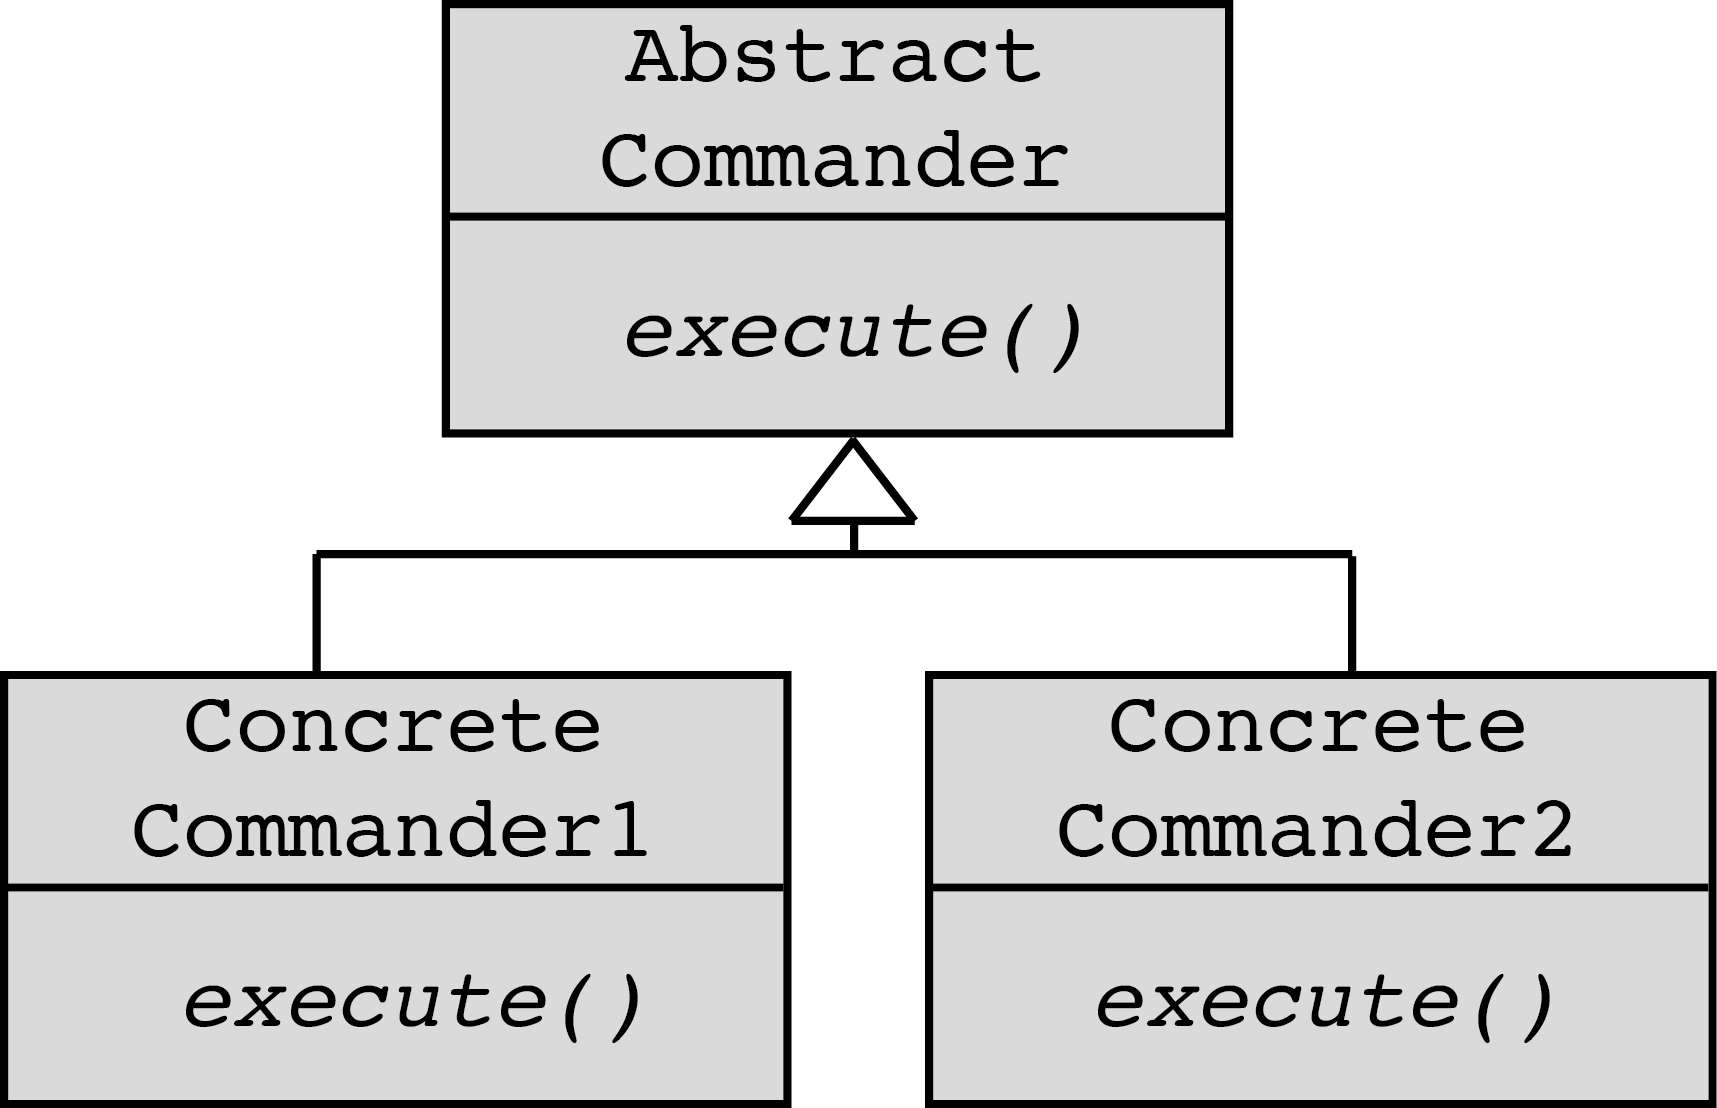
\includegraphics[keepaspectratio=true,scale=0.4]{./Commander/Commander}
\end{SCfigure}
Sometimes we need to wrap a snippet of code in a container to be executed later at a given instruction. The \textbf{Commander} pattern is tailored for this situation. When you use this pattern, you are no longer telling, ``Do this''; instead you are saying, ``Remember how to do this,'' and, sometime later ``Do that thing I told you to remember''. The two-part aspect of this pattern adds some serious complexity to the code and we have to make sure that we really need that additional complexity. Before we introduced commanders in the SIMPLE library, SIMPLE was a scattered mess of little command-line-driven programs that were really only usable by us (the developers) and a few other brave souls that needed to use it because nothing else worked. I wanted to preserve the flexibility that finely chopped functionality gives and in the same time allow creation of higher level workflows, all within the Fortran environment. The solution came from the commander pattern. By making every little program a commander and splitting up many of the most aggregated programs into smaller units, we preserved (and even increased) the flexibility while simultaneously allowing the creation of higher level workflows via execution of many commanders in sequence. This is how it works:
\begin{verbatim}
module simple_commander_base
implicit none

public :: commander_base
private

type, abstract :: commander_base
  contains
    procedure(generic_execute), deferred :: execute
end type commander_base

abstract interface

    !>  \brief  executes the commander
    subroutine generic_execute( self, cline )
        use simple_cmdline, only: cmdline
        import :: commander_base
        class(commander_base), intent(inout) :: self
        class(cmdline), intent(inout)        :: cline
    end subroutine generic_execute

end interface

end module simple_commander_base
\end{verbatim}
The abstract base class defines the common interface, consisting of the instance (self) and a command line implemented as object. The command line may now come from parsing the actual command line or creating command line objects from within the environment to control execution. The single method \texttt{execute} executes the code that is implemented in the concrete commander (a type extension of this abstract base class). This is an example of a concrete commander:
\begin{verbatim}
module simple_commander_imgproc
use simple_defs            ! singleton
use simple_jiffys          ! singleton
use simple_cmdline,        only: cmdline
use simple_params,         only: params
use simple_build,          only: build
use simple_commander_base, only: commander_base
implicit none

public :: convert_commander
private

type, extends(commander_base) :: convert_commander
  contains
    procedure :: execute      => exec_convert
end type convert_commander

    subroutine exec_convert( self, cline )
        class(convert_commander), intent(inout) :: self
        class(cmdline),           intent(inout) :: cline
        type(params), target :: p
        type(build),  target :: b
        integer              :: iptcl
        p = params(cline, allow_mix=.true.) ! parameters generated
        call b%build_general_tbox(p, cline) ! general objects built
        if( cline%defined('stk') )then
            do iptcl=1,p%nptcls
                call progress(iptcl, p%nptcls)
                call b%img%read(p%stk, iptcl)
                call b%img%write(p%outstk, iptcl)
            end do 
        else if( cline%defined('vol1') )then
            call b%vol%read(p%vols(1))
            call b%img%write(p%outvol)
        else
            stop 'either vol1 or stk argument required to execute simple_convert'
        endif
        ! end gracefully
        call simple_end('**** SIMPLE_CONVERT NORMAL STOP ****')
    end subroutine exec_convert
\end{verbatim}
This commander converts between SPIDER and MRC format files and vice versa.

\subsection{SIMPLE Modules}
Modules are an old, established design element that plays a key role in modern Fortran. The Fortran module is technically implementing a singleton design pattern, \textit{i.e.} there can be only one instance of a module, it does not need to be instantiated and the data declared in the header of the module (not in the subroutines and functions) exist throughout the execution of the program. Everyone uses modules but few treat them as a full-fledged part of the model. Code gets broken down into all sorts of categories, from aspects of the technical architecture to developers' work assignments. Even developers who refactor a lot tend to content themselves with modules conceived early in the project.

It is a truism that there should be low coupling between modules and high cohesion within them. Explanations of coupling and cohesion tend to make them sound like technical metrics, to be judged mechanically based on the distributions of associations and interactions. Yet it isn't just code being divided into modules, but concepts. There is a limit to how many things a person can think about at once (hence low coupling). Incoherent fragments of ideas are as hard to understand as an undifferentiated soup of ideas (hence high cohesion). Well-chosen modules bring together elements of the model with particularly rich conceptual relationships. This high cohesion of objects with related responsibilities allows modelling and design work to concentrate within a single module, a scale of complexity a human mind can easily handle. When you place some classes together in a module, you are telling the next developer who looks at your design to think about them together, as a team working together toward a common goal. If your model is telling a story (about how to process single-particle images), the modules are chapters.

\textbf{Choose modules that tell a story about the system and contain a cohesive set of concepts. This often yields low coupling between modules, but if it doesn't, look for a way to change the model to disentangle the concepts, or search for an overlooked concept that might be the basis of a module that would bring elements together in a meaningful way. Seek low coupling in the sense of concepts that can be understood and reasoned about independently of each other. Refine the model until it partitions according to high-level domain concepts and the corresponding code is decoupled as well.}

Give modules names that become part of the \textit{ubiquitous language}. Modules and their names should reflect insight into the domain. In SIMPLE, we have two kinds of modules. (1) Modules defining constants that need to be available via the \texttt{use} statement, for example:
\begin{verbatim}
module simple_defs
use, intrinsic :: iso_c_binding
implicit none
! 'I', 'M' or 'S' for imagic, mrc, spider
character(len=1), parameter :: default_file_format = 'M' 
integer, parameter  :: IMPORTANT=10 ! number of solutions considered important
integer, parameter  :: MAXS=20      ! maximum number of states
integer, parameter  :: STDLEN=256   ! standard string length
integer, parameter  :: short = selected_int_kind(4)
integer, parameter  :: long  = selected_int_kind(9)
integer, parameter  :: longer  = selected_int_kind(16)
integer, parameter  :: I4B = SELECTED_INT_KIND(9)
integer, parameter  :: I2B = SELECTED_INT_KIND(4)
integer, parameter  :: I1B = SELECTED_INT_KIND(2)
integer, parameter  :: SP = KIND(1.0)
integer, parameter  :: DP = KIND(1.0D0)
integer, parameter  :: DOUBLE = KIND(1.0D0)
integer, parameter  :: SPC = KIND((1.0,1.0))
integer, parameter  :: DPC = KIND((1.0D0,1.0D0))
integer, parameter  :: LGT = KIND(.true.)
integer, parameter  :: line_max_len = 8192 !< Max number of characters on line
real(sp), parameter :: PI=acos(-1.)
real(sp), parameter :: PIO2=acos(-1.)/2.
real(sp), parameter :: TWOPI=2.*acos(-1.)
real(sp), parameter :: FOURPI=4.*acos(-1.)
real(sp), parameter :: SQRT2=sqrt(2.)
real(sp), parameter :: EUL=0.5772156649015328606065120900824024310422_sp
real(sp), parameter :: um2a = 10000.
real(sp), parameter :: TINY=1e-10
real(sp), parameter :: SMALL=1e-6
real(sp), parameter :: MINEULSDEV=3.
real(sp), parameter :: MINTRSSDEV=0.5
real(sp), parameter :: FTOL=1e-4
real(dp), parameter :: DTINY=1e-10
real(dp), parameter :: DSMALL=1e-6
real(dp), parameter :: pisqr = PI*PI   ! PI^2.

! plan for the CTF
type :: ctfplan
    character(len=STDLEN) :: mode='' !< astig/noastig
    character(len=STDLEN) :: flag='' !< flag: <mul|flip|no> 
end type ctfplan

! the c binding derived type for the system query module
type, bind(c) :: systemDetails
   integer(c_int) :: n_phys_proc
   integer(c_int) :: nCPUcores
#if defined (MACOSX)   
   integer(c_int64_t) :: mem_Size
   integer(c_int) :: mem_User
#elif defined (LINUX)
   integer(c_long_long) :: mem_Size
   integer(c_long_long) :: avail_Mem
#else
   integer(c_int)     :: mem_size
#endif
end type systemDetails

! endianness conversion
character(len=:), allocatable :: endconv

! number of threads global variable
integer(kind=c_int):: nthr_glob

end module simple_defs
\end{verbatim}
and (2) modules that implement high-level functionalities (look at the \texttt{simple\_hadamard2D\_matcher} and \texttt{simple\_hadamard3D\_matcher} for examples).

\section{Refactoring Toward Deeper Insight}

\subsection{Making Implicit Concepts Explicit}
A deep, well-constructed model has power because it contains the central concepts and abstractions that can succinctly and flexibly express essential knowledge of the user's activities, their problems, and their solutions. The first step is to somehow represent the essential concepts of the domain in the model. Refinement comes later, after successive iterations of knowledge crunching and refactoring. But this process really gets into gear when an important concept is recognised and made explicit in the model and design.

\textbf{Many transformations of domain models and the corresponding code happens when developers recognise a concept that has been hinted at in discussion or present implicitly in the design, and they then represent it explicitly in the model with one or more objects or relationships.}

Listen to the language the domain experts (the electron microscopists) use. Are there terms that succinctly state something complicated? Are they correcting your word choice (perhaps diplomatically)? Do the puzzled looks on their faces go away when you use a particular phrase? These are hints of a concept that will for sure benefit the model. When the users or domain experts use vocabulary that is nowhere in the design, that's a warning sign. It is a doubly strong warning when both the developers and the domain experts are using terms that are not in the design.

\subsection{Supple Design}
Supple is an adjective that means ``bending and moving easily and gracefully; flexible''. The ultimate purpose of software is to serve users. But first, that same software has to serve developers. This is especially true in a process that emphasises refactoring. I assume here that the reader knows that refactoring entails much more than simply renaming functions and subroutines. Refactoring is the process of moving bits and pieces of code around, making it logically consistent, readable and naming consistent with the domain model. This should be done without changing the program's external behaviour. Succesful refactoring strongly depends on having well-designed automatic unit tests (discussed below). Ruthless refactoring is a key component of the extreme programming paradigm and it is best done in paris, with one coder overlooking the shoulder of the other.

\textbf{When software doesn't have a clean design, developers dread even looking at the existing mess or making a change that could aggravate the tangle or break something through an unforeseen dependency. To have a project accelerate as development proceeds\textemdash{}rather than get weighted down by its own legacy\textemdash{}demands a design that is a pleasure to work with, inviting to change. A supple design.}

A lot of overengineering has been justified in the name of flexibility. How do you structure an application or a framework so that it is extensible, so that other engineers can easily add bits to it as the program evolves over time? As we construct an even more ambitious system, the problem of making it configurable and extensible looms even larger. Look at the design of software that really empowers the people who handle it; you will usually see something simple. Simple is not easy. To create elements that can be assembled into elaborate systems and still be understandable, a dedication to \textit{model-driven design} has to be joined with a moderately rigorous design style. Good programmers value simplicity, and the simple thing to do here is to rigorously cancel out all unnecessary flexibility. If you have no use for it, flexibility becomes a danger. We want to preserve the essential extensibility of our framework, yet get rid of the extraneous configuration. The idea with this document and the object-oriented SIMPLE design is to provide you\textemdash{}the developer\textemdash{}with a template that emphasises convention over configuration.

\begin{SCfigure}[][h]
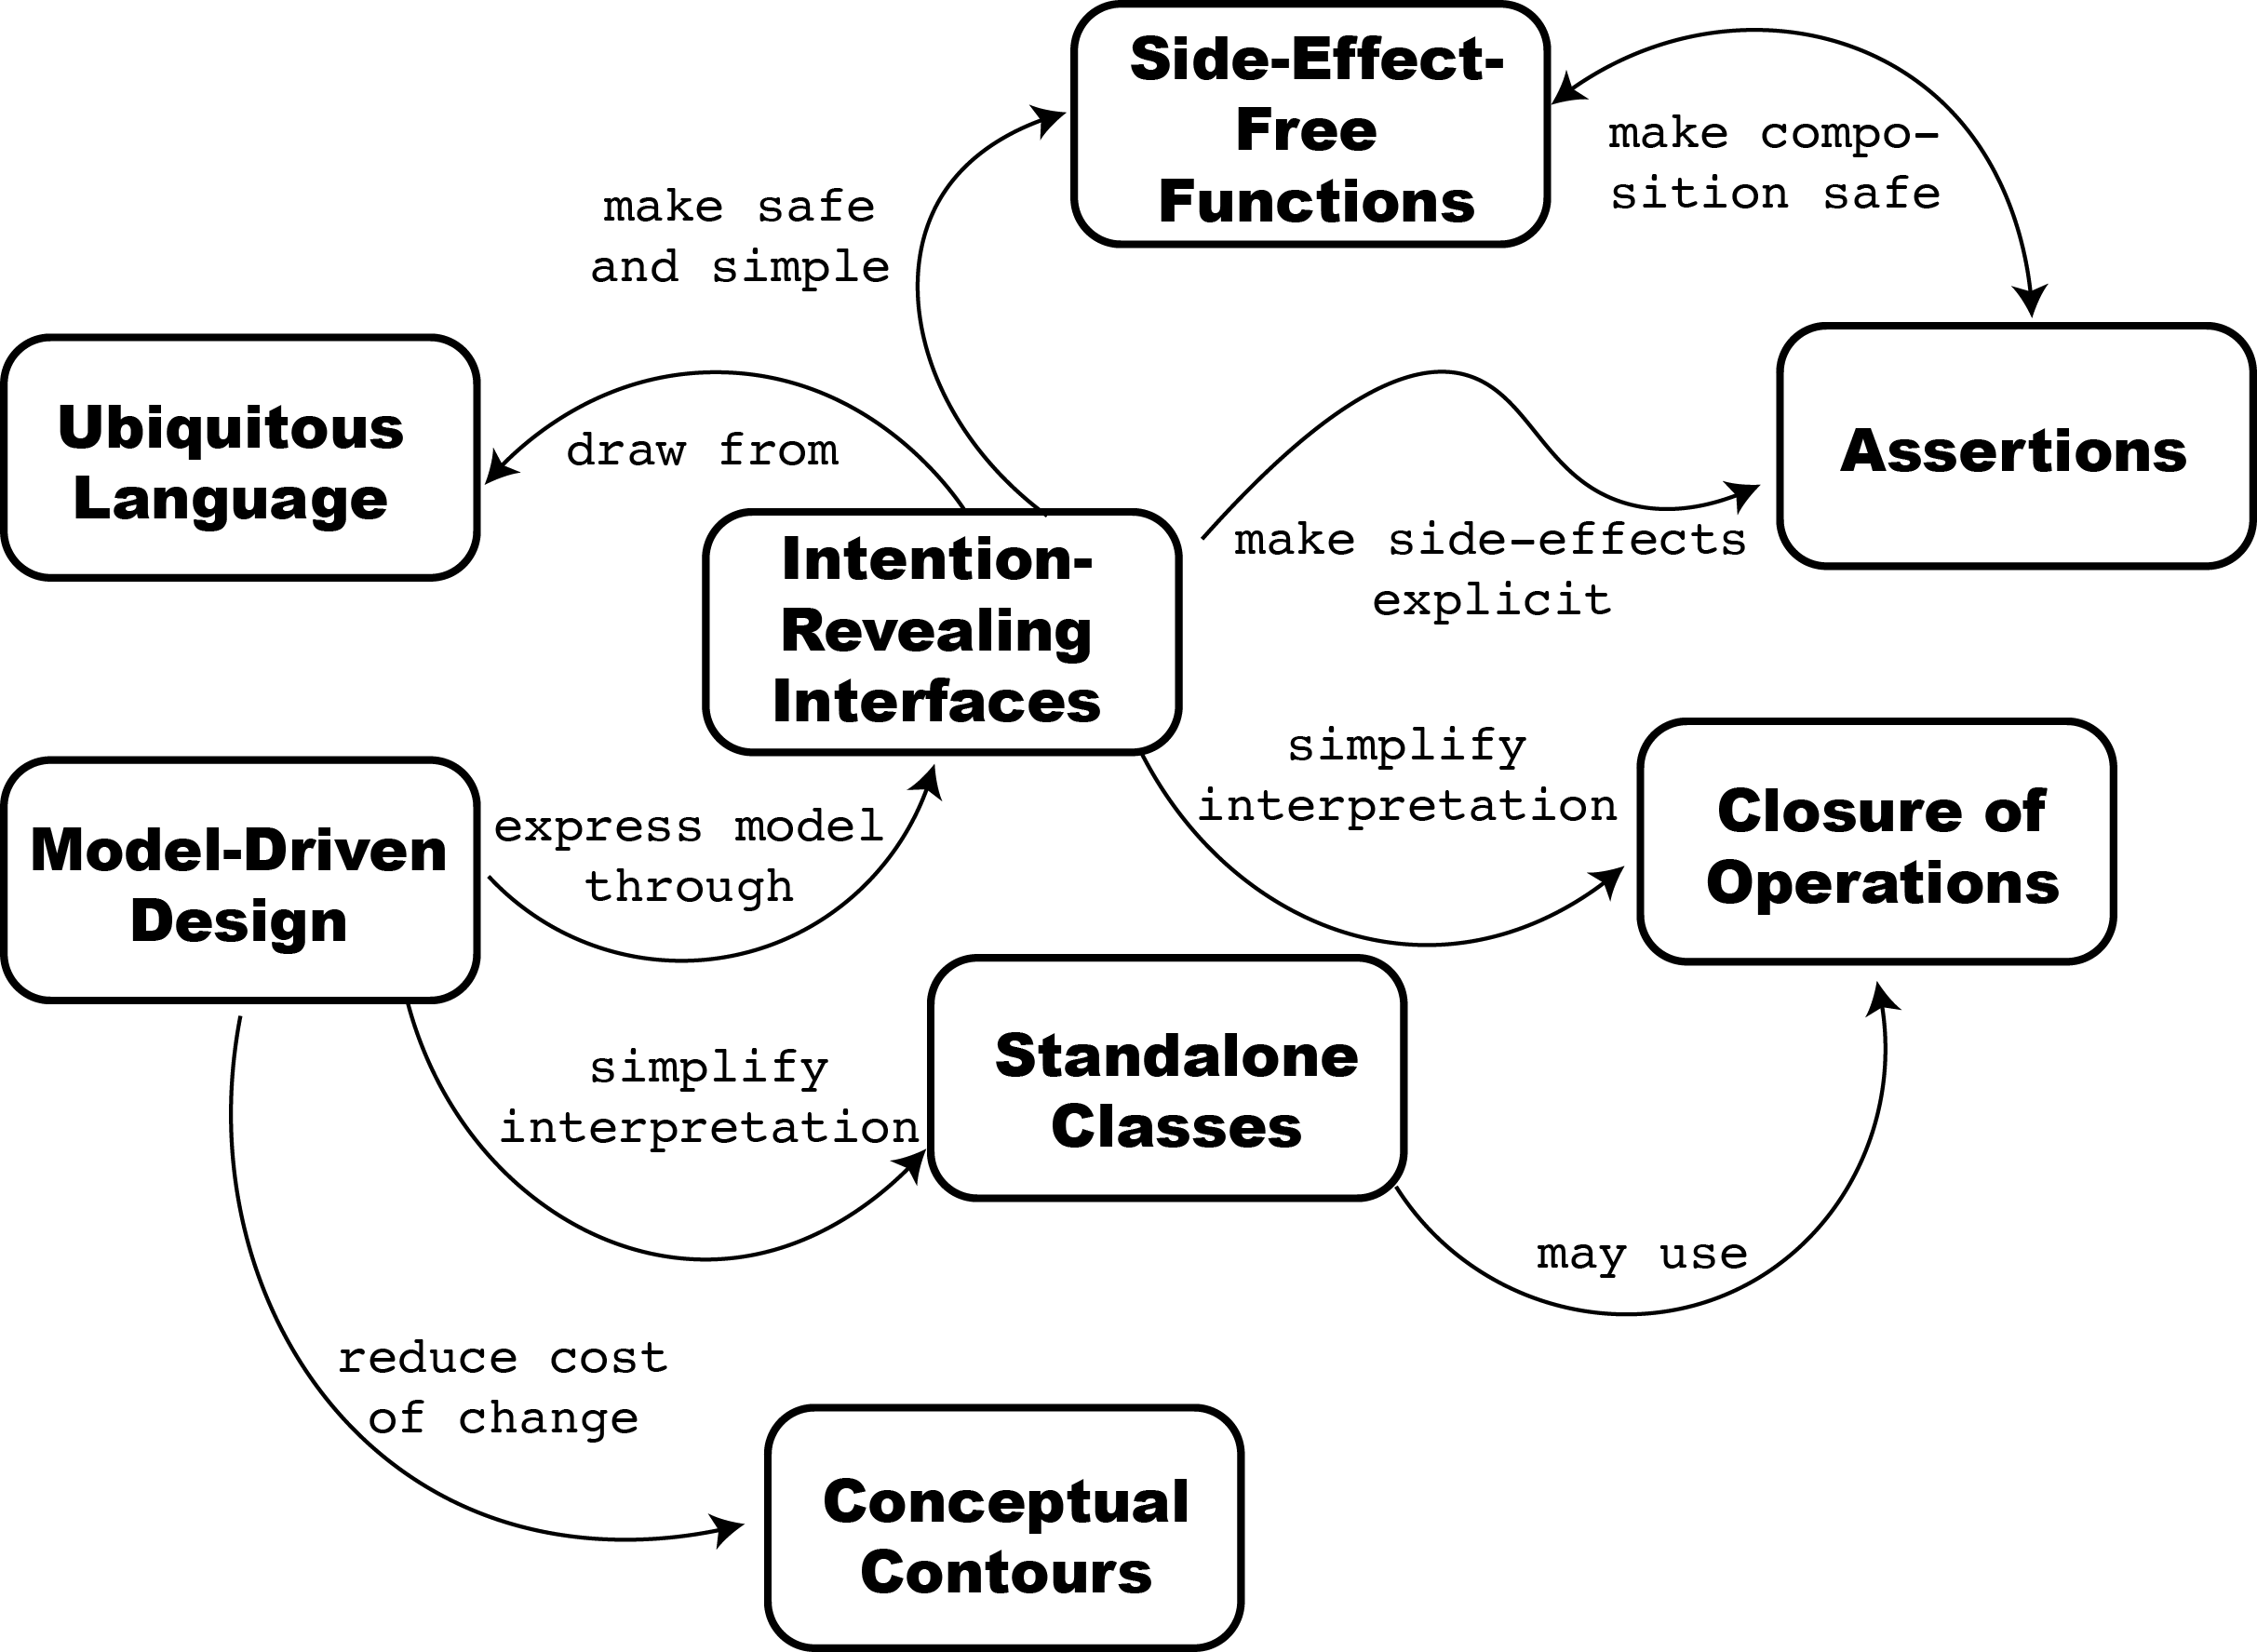
\includegraphics[keepaspectratio=true,scale=0.6]{./SuppleDesign/SuppleDesign}
\caption{Some patterns that contribute to supple design.}
\end{SCfigure}

\subsection{Intention-Revealing Interfaces}
If a developer must consider the implementation of a component in order to use it, the value of encapsulation is lost. If someone other than the original developer must infer the purpose of an object or operation based on its implementation, that new developer may infer a purpose that the operation or class fulfils only by chance. If that was not the intent, the code may work for a moment, but the conceptual basis of the design will have been corrupted, and the two developers will be working at cross-purpose.

Name classes and operations to describe their effect and purpose, without reference to the means by which they do what they promise. This relieves the client of the need to understand the internals. These names should conform to the \textit{ubiquitous language} so that team members can quickly infer their meaning. I tend to try to keep names short, not because my limited memory prevents me to use long method names, but because the code becomes a mess to read when names are too long.

\subsection{Side-Effect-Free Functions}
Place as much of the logic of a program into functions, operations that return results with no observable side-effects. This can be enforced by the use of pure and elemental functions in modern Fortran (example below)

\begin{verbatim}
!>  \brief  this metric is measuring the frobenius deviation from the identity
!!          matrix .in.[0,2*sqrt(2)] Larochelle, P.M., Murray, A.P., Angeles, J., 
!!          A distance metric for finite sets of rigid-body displacement in the 
!!          polar decomposition. ASME J. Mech. Des. 129, 883?886 (2007)
pure real function geodesic_dist( self1, self2 )
    class(ori), intent(in) :: self1, self2
    real :: Imat(3,3), sumsq, diffmat(3,3)
    Imat      = 0.
    Imat(1,1) = 1.
    Imat(2,2) = 1.
    Imat(3,3) = 1.
    diffmat = Imat-matmul(self1%rmat,transpose(self2%rmat))
    sumsq   = sum(diffmat*diffmat)
    if( sumsq > 0.0001 )then
        geodesic_dist = sqrt(sumsq)
    else
        geodesic_dist = 0.
    endif
end function geodesic_dist
\end{verbatim}

Strictly segregate commands (methods that result in modifications to observable state) into very simple operations that do not return domain information. Further control side effects by moving complex logic into \textit{value objects} when a concept fitting the responsibility presents itself.

\subsection{Assertions}
In contrast to for example Java or C++, Fortran isn't really equipped with any good tools to deal with assertions and Fortran programmers generally feel uneasy when plowing through code scattered with assert statements. In SIMPLE, we have never coded assertions directly into our classes. Instead, we rely on a set of automated unit tests (described below) which admittedly needs to be extended to test more code than it currently does. 

\subsection{Conceptual Contours}
Sometimes developers chop functionality fine to allow flexible combination. Sometimes they lump it large to encapsulate complexity. Sometimes they seek a consistent granularity, making all classes and operations to a similar scale. These are oversimplifications that don't work well as a general rule. As a rule of thumb, if your method call has more than three arguments (excluding the object instance), chances are you are lumping it too large. On the other hand, when performance is important and the embedded algorithm will be subjected to parallelisation, substantial performance gains may follow from merging operations and reduce overheads due to thread creation, data transfer to devices etc. However, remember the famous quote by Donald Knuth ``Premature optimisation is the root of all evil''. Therefore:

\textbf{Decompose design elements (operations, interfaces, classes and aggregates) into cohesive units, taking into consideration your intuition of the important divisions in the domain. Observe the axes of change and stability through successive refactorings and look for the underlying \textit{conceptual contours} that explain these shearing patterns. Align the model with the consistent aspects of the domain that make it a viable area of knowledge in the first place.}

The goal is a simple set of interfaces that combine logically to make sensible statements in the \textit{ubiquitous language}, and without the distraction and maintenance burden of irrelevant options. This is typically an outcome of refactoring: it's hard to produce up front. But it may never emerge from technically oriented refactoring; it emerges from refactoring toward deeper insight. The \texttt{simple\_ctf} class is an example of a successfully encapsulated functionality. It also represents a standalone class (discussed below).

\begin{verbatim}
module simple_ctf
use simple_defs ! singleton
implicit none

public :: ctf, test_ctf
private

type ctf
    private
    real    :: smpd        = 0.    !< sampling distance (A)
    real    :: kV          = 0.    !< acceleration voltage (kV) 
    real    :: Cs          = 0.    !< spherical aberration (mm)
    real    :: wl          = 0.    !< wavelength (A)
    real    :: amp_contr   = 0.07  !< fraction of amplitude contrast ([0.07,0.15])
    real    :: dfx         = 0.    !< underfocus x-axis (microns)
    real    :: dfy         = 0.    !< underfocus y-axis (microns)
    real    :: angast      = 0.    !< azimuth of x-axis 0.0 means (degrees)
    real    :: phaseq      = 0.    !< phase contrast weight (derived constant)
    real    :: ampliq      = 0.    !< amplitude contrast weight (derived constant)
  contains
    ! INITIALISER
    procedure, private :: init
    ! CTF EVALUATION
    procedure          :: eval
    procedure, private :: evalPhSh
    procedure, private :: eval_df
    ! CTF APPLICATION
    procedure          :: ctf2img
    procedure          :: ctf2spec
    procedure          :: apply
    ! CALCULATORS
    procedure          :: freqOfAZero
    procedure, private :: solve4PhSh
    procedure, private :: sqFreq4PhSh
    procedure, private :: sqSf4PhSh
end type

interface ctf
    module procedure constructor
end interface
\end{verbatim}

\subsection{Standalone Classes}
\textbf{Even within a module, the difficulty of interpreting a design increases wildly as dependencies are added. This adds to mental overload, limiting the design complexity a developer can handle. Implicit concepts contribute to this load even more than explicit references.}

Refined models are distilled until every remaining connection between concepts represents something fundamental to the meaning of those concepts. In an important subset, the number of dependencies can be reduced to zero, resulting in a class that can be understood all by itself, along with a few primitives and basic library concepts.

\textbf{Low coupling is fundamental to object design. When you can, go all the way. Eliminate \textit{all} other concepts from the picture. Then the class will be completely self-contained and can be studied and understood alone. Every such self-contained class significantly eases the burden of understanding a module.}

Dependencies on other classes within the same module is less harmful than those outside. Likewise, when two objects are naturally tightly coupled, multiple operations involving the same pair can actually clarify the relationship. The goal is not to eliminate all dependencies, but to eliminate all nonessential ones.

\section{Maintaining Model Integrity}
Although we seldom think about it explicitly, the most fundamental requirement of a model is that it be internally consistent; that its terms always have the same meaning, and that it contains no contradictory rules. The internal consistency of a model, such that each term is unambiguous and no rules contradict, is called \textit{unification}. A model is meaningless unless it is logically consistent. In an ideal world, we would have a single model spanning the whole domain of the research field. This model would be unified, without any contradictory or overlapping definitions of terms. Every logical statement about the domain would be consistent. 

\subsection{Continuous Integration}
It is very hard to maintain the level of communication needed to develop a unified system of any size. We need ways of increasing communication and reducing complexity. We also need safety nets that prevent overcautious behaviour, such as developers duplicating functionality because they are afraid that they will break existing code. Of equal importance to prevent such undesired behaviours is that all developers are reaching a certain level of understanding of the system. Naturally, certain developers will have areas where they excel but there is a knowledge threshold that all the developers in the team must pass. We also need to respect the rules of the framework and in the same time not being afraid of introducing changes. It is a delicate balance. The team must cultivate a shared understanding of the ever-changing model. Practices may help, but the most fundamental one is to constantly update the \textit{ubiquitous language} definition. SIMPLE developers use Git for step-by-step, reproducible merge/build and automated test suites (both described below). Development sometimes occurs in spurts and sometimes stagnates, depending on the current workload of the team. However, we must strive to merge all code frequently and relentlessly exercise the  \textit{ubiquitous language} to hammer out a shared view of the model as the concepts evolve in different people's heads.

\section{The SIMPLE Compilation Environment}
Although seldom discussed in length in any programming books, an effective method for code compilation is crucial. The developer that repeatedly needs to re-compile/test/re-compile/test/re-compile... would soon go mad with a clumsy time-consuming compilation environment. Fortran is particularly tricky to compile as order matters to a much larger extent than in C or C++ and circular references are not supported. We have therefore developed our own compilation environment based on a combo of shellscripts, makefiles and perl. 

\subsection{\texttt{Makefile\_target} Files and Makefile Generation with \texttt{makemake}}
If you execute \texttt{ls} is the SIMPLE root directory, you see something like
\begin{verbatim}
@!#> ls
Makefile                 compileSIMPLE.pl*        obj/                     src/
Makefile_macros          defs/                    production/              test_code/
README.txt               doc/                     scripts/                 web/
add2.bashrc              examples/                simple_distr_config.env
add2.tcshrc              legacy/                  simple_user_input.pm*
bin/                     makemake*                simple_utils/
\end{verbatim}
Every folder that contains code that should be part of the build or folders with code that should be part of the build contains a file called \texttt{Makefile\_target}. The simplest example is the \texttt{defs/} folder
\begin{verbatim}
@!#> cd defs/
@!#> ls
Makefile_target   simple_defs.f90   simple_fftw3.f90
@!#> cat Makefile_target 
defs_code: simple_defs.o   \
           simple_fftw3.o  ;
\end{verbatim}
Now, say that I develop a new module with definitions for cuda \texttt{simple\_cuda\_defs} that uses (depends on) \texttt{simple\_defs} but does not use \texttt{simple\_fftw3}. I would then update \texttt{Makefile\_target} to either
\begin{verbatim}
defs_code: simple_defs.o      \
           simple_cuda_defs.o \
           simple_fftw3.o     ;
\end{verbatim}
or
\begin{verbatim}
defs_code: simple_defs.o      \
           simple_fftw3.o     \
           simple_cuda_defs.o ;
\end{verbatim}
but NOT to
\begin{verbatim}
defs_code: simple_cuda_defs.o \
           simple_defs.o      \
           simple_fftw3.o     ;
\end{verbatim}
as compilation would fail. There are more complex examples, such as the \texttt{src/simple\_main} folder (the curious reader may now have a look). However, the principle is the same. We define a compilation hierarchy that ensures that all dependencies are satisfied. The \texttt{makemake} shellscript uses all the \texttt{Makefile\_target} files in the library to create a common makefile. \texttt{makemake} scans directories, sub-directories and sub-sub-directories, so we never make directory structures more than three levels deep. If you introduce new code and update the \texttt{Makefile\_target} files, you need to re-make the make file by executing \texttt{makemake} in the SIMPLE root directory. The \texttt{makemake} script should not be modified by others than Hans.

\subsection{The \texttt{compileSIMPLE.pl} script}
In addition to the makefile we need to define compilation macros informing the makefile about the SIMPLE root directory, which compilation switches to use, which compilers to use, if there are paths that contain libraries to link to, where the object and module files are going to be located, which compilers to use and what compiler flags to include. Moreover, we have scripts that autogenerate code and/or modify code that needs to be executed. All of this is taken care of by \texttt{compileSIMPLE.pl} located in the SIMPLE root directory. Once you have a healthy makefile, you execute \texttt{compileSIMPLE.pl} to compile the suite and following succesful compilation you see something like
\begin{verbatim}
@!#> ./compileSIMPLE.pl 
*********************************************************
* Checking and printing the input directories...        *
*********************************************************
SIMPLE_PATH          : /Users/hael/src/fortran/simple3.0
SIMPLE_SRC_PATH      : /Users/hael/src/fortran/simple3.0/src/simple_main
SIMPLE_PROD_PATH     : /Users/hael/src/fortran/simple3.0/production
SIMPLE_TEST_PROD_PATH: /Users/hael/src/fortran/simple3.0/production/simple_tests
SIMPLE_SCRIPTS_PATH  : /Users/hael/src/fortran/simple3.0/scripts
*********************************************************
Moving to dir: /Users/hael/src/fortran/simple3.0/src/simple_main
Executing simple_args_generator.pl in dir: /Users/hael/src/fortran/simple3.0...
Moving to dir: /Users/hael/src/fortran/simple3.0
Generating Makefile_macros: /Users/hael/src/fortran/simple3.0
/sw/bin/gfortran -c -fimplicit-none -fall-intrinsics -ffree-form -cpp -fpic...
...
sw/bin/gfortran -c -fimplicit-none -fall-intrinsics -ffree-form -cpp -fpic... 

darwin, Platform = 0
Architecture: darwin-thread-multi-2level

Moving to dir: /Users/hael/src/fortran/simple3.0/production
Generating compile_and_link: /Users/hael/src/fortran/simple3.0/production
Moving to dir: /Users/hael/src/fortran/simple3.0
Compiling production codes:
>>> COMPILING & LINKING: simple_test_volpft_srch
>>> COMPILING & LINKING: simple_test_cartcorr_sanity
>>> COMPILING & LINKING: simple_test_ft_expanded
>>> COMPILING & LINKING: simple_test_sysparse
>>> COMPILING & LINKING: simple_test_units
>>> COMPILING & LINKING: simple_distr_exec
>>> COMPILING & LINKING: simple_test_picker
>>> COMPILING & LINKING: simple_test_clineparse
>>> COMPILING & LINKING: simple_test_srch
>>> COMPILING & LINKING: simple_test_shelliter
>>> COMPILING & LINKING: simple_exec
>>> COMPILING & LINKING: simple_test_imgfile
>>> COMPILING & LINKING: simple_test_scatsrch
Compilation of SIMPLE completed in dir: /Users/hael/src/fortran/simple3.0
\end{verbatim}
The \texttt{compileSIMPLE.pl} script should not be modified by others than Hans. However, the perl module \texttt{simple\_user\_input.pm} containing all the definitions that \texttt{compileSIMPLE.pl} uses needs to be modified to suit the architecture that SIMPLE is being compiled on. Editing \texttt{simple\_user\_input.pm} should be straightforward, but if you have questions talk to Cyril or Hans.

\section{The SIMPLE Test Environment}
Test-driven development is a key component of the extreme programming paradigm, which advocates writing the test code before you are writing the code that passes the test. I have never fully adopted this idea, because scientific programming often involves a defined enough problem to solve that you can just get on with it. We are certainly not going to try to live up to the software industry in terms of test rigour, but we have a few SIMPLE test guidelines. 

\subsection{One Class, One Unit Test}
When you implement a new class, implement a unit test for that class in the end of the module, after the destructor. Fortran allows you to implement subroutines and functions that are not type-bound within the module that defines the class, which can be very convenient but should not be abused (unit tests is an acceptable reason). Take the \texttt{simple\_ori} (orientation) class as example:
\begin{verbatim}
module simple_ori
use simple_defs  ! singleton
use simple_hash,   only: hash
use simple_jiffys, only: alloc_err
implicit none

public :: ori, test_ori, test_ori_dists
private

real, parameter    :: zvec(3)=[0.,0.,1.]

!>  \brief  orientation parameters
type :: ori
    private
    real                        :: euls(3)=0.        !< Euler angle
    real                        :: normal(3)=0.      !< Fourier plane normal
    real                        :: rmat(3,3)=0.      !< rotation matrix
    type(hash)                  :: htab              !< hash table for the parameters
    logical                     :: existence=.false. !< to indicate existence
  contains
    ! CONSTRUCTOR
    procedure          :: new_ori
    procedure          :: new => new_ori
    ...
\end{verbatim}
\texttt{simple\_ori} implements two unit tests: \texttt{test\_ori} and \texttt{test\_ori\_dists} that are made public together with object. All unit tests come together in the executable \texttt{simple\_test\_units}, located in  \texttt{/production/simple\_tests/simple\_test\_units}, which represents the low-level test routine in SIMPLE. 

\subsection{The High-Level Test Environment}
In addition to the low-level unit tests, we need a high-level testing environment that can test modules and interactions between classes. This environment is located in the \texttt{test\_code/} folder. High-level tests are implemented as modules. The cpu test code is located in \texttt{test\_code/cpu}
\begin{verbatim}
@!#> cd test_code/cpu/
@!#> ls
Makefile_target                    simple_prime2D_srch_tester.f90
simple_ft_expanded_tester.f90      simple_prime3D_srch_tester.f90
simple_optimiser_tester.f90        simple_scatter_orisrch_tester.f90
\end{verbatim}
Please study these modules to understand how high-level tester code is implemented. Often, high-level tests require input, such as images or volumes, and a binary executable needs to be created. For example:
\begin{verbatim}
@!#> cd production/simple_tests/simple_test_srch/
@!#> cat simple_test_srch.f90 
program simple_test_srch
use simple_prime2D_srch_tester
use simple_wiener2D_tester
use simple_optimiser_tester
use simple_prime3D_srch_tester
use simple_volpft_srch_tester
use simple_cmdline, only: cmdline
implicit none
type(cmdline) :: cline
logical       :: be_verbose=.false.
if( command_argument_count() < 3 )then
    write(*,'(a)',advance='no') 'simple_test_srch vol1=<volume.mrc> msk=<mask radius(in pixels)>'
    write(*,'(a)') ' smpd=<sampling distance(in A)> [nthr=<number of threads{1}>] [verbose=<yes|no{no}>]'
    stop
endif
call cline%parse
call cline%checkvar('vol1', 1)
call cline%checkvar('msk',  2)
call cline%checkvar('smpd', 3)
call cline%check
be_verbose = .false.
if( cline%defined('verbose') )then
    if( trim(cline%get_carg('verbose')) .eq. 'yes' )then
        be_verbose = .true.
    endif
endif
call exec_prime2D_srch_test( cline, be_verbose )
call exec_prime3D_srch_test( cline, be_verbose )
call exec_wiener2D_test    ( cline, be_verbose )
call exec_optimiser_test   (        be_verbose )
end program simple_test_srch
\end{verbatim}
implements the high-level search tests.

\section{Distributing SIMPLE on Workstations and Clusters}
We never had any dedicated distributing computing environment to run our code on but were always part of multi-user queue systems. Creating an MPI applications that asks for a large number of processors for a long time was therefore not an option for us, as our job would have spent most of the time idling. Instead, we hacked the job submission system. The original environment was built in perl, but we have now transferred it all into the Fortran environment. Most simple executables (executed with \texttt{simple\_exec}) accepts the command line parameters \texttt{nparts}, \texttt{part}, \texttt{fromp} and \texttt{top} indicating the number of partitions, the partition number and the from/to range of particles to be processed by the \texttt{part} partition. The driver code creates balanced partitions and scripts that are executed by the queue system. Currently we support PBS, SLURM and local, where local is the execution method for workstations without any job submission system installed. To understand how it is done, please study the \texttt{simple\_qsys*} classes. \texttt{simple\_qsys\_ctrl} is the scheduler that supports asynchronous execution of \texttt{nparts} partitions over a given number of computational units \texttt{ncunits}. We use an abstract factory for defining the different environments. This is a good example of the principle of separating the things that change from the ones that stay the same. The abstract base class defines the interface (remember the gang of four's advice ``code to an interface, not to an implementation'')
\begin{verbatim}
module simple_qsys_base
implicit none

public :: qsys_base
private

type, abstract :: qsys_base
  contains
    procedure(generic_new),         deferred :: new
    procedure(generic_submit_cmd),  deferred :: submit_cmd
    procedure(generic_write_instr), deferred :: write_instr
    procedure(generic_kill),        deferred :: kill
end type qsys_base

abstract interface

    !>  \brief  constructor
    subroutine generic_new( self )
        import :: qsys_base
        class(qsys_base), intent(inout) :: self
    end subroutine generic_new
    
    !>  \brief  getter that returns the submit command of the qsys
    function generic_submit_cmd( self ) result ( submit_cmd )
        import :: qsys_base
        class(qsys_base), intent(in)  :: self
        character(len=:), allocatable :: submit_cmd
    end function generic_submit_cmd
    
    !>  \brief  writes a header instruction for the submit script
    subroutine generic_write_instr( self, job_descr, fhandle )
        use simple_chash, only: chash
        import :: qsys_base
        class(qsys_base),  intent(in) :: self
        class(chash),      intent(in) :: job_descr
        integer, optional, intent(in) :: fhandle   
    end subroutine generic_write_instr

    !>  \brief  destructor
    subroutine generic_kill( self )
        import :: qsys_base
        class(qsys_base), intent(inout) :: self
    end subroutine generic_kill
    
end interface

end module simple_qsys_base
\end{verbatim}
and the concrete type extended classes define the different job submission environments (see class for SLURM-based execution below).
\begin{verbatim}
module simple_qsys_slurm
use simple_qsys_base, only: qsys_base
use simple_chash,     only: chash
implicit none

public :: qsys_slurm
private

integer, parameter :: MAXENVITEMS=100

type, extends(qsys_base) :: qsys_slurm
    private
    type(chash) :: env !< defines the SLURM environment
  contains
    procedure :: new         => new_slurm_env
    procedure :: submit_cmd  => get_slurm_submit_cmd
    procedure :: write_instr => write_slurm_header
    procedure :: kill        => kill_slurm_env
end type qsys_slurm

contains
    
    !> \brief  is a constructor
    subroutine new_slurm_env( self )
        class(qsys_slurm), intent(inout) :: self
        ! make the container
        call self%env%new(MAXENVITEMS)
        ! define the environment:
        ! ### USER PARAMETERS
        call self%env%push('user_account',          '#SBATCH --account')
        call self%env%push('user_email',            '#SBATCH --mail-user')
        ! ### QSYS PARAMETERS
        call self%env%push('qsys_partition',        '#SBATCH --partition')
        call self%env%push('qsys_qos',              '#SBATCH --qos')
        call self%env%push('qsys_reservation',      '#SBATCH --reservation')
        call self%env%push('qsys_submit_cmd',       'sbatch')
        ! ### JOB PARAMETERS
        call self%env%push('job_name',              '#SBATCH --job-name')
        call self%env%push('job_ntasks',            '#SBATCH --ntasks')
        call self%env%push('job_ntasks_per_socket', '#SBATCH --ntasks-per-socket')
        call self%env%push('job_cpus_per_task',     '#SBATCH --cpus-per-task') 
        call self%env%push('job_memory_per_task',   '#SBATCH --mem')
        call self%env%push('job_time',              '#SBATCH --time')
    end subroutine new_slurm_env

    !> \brief  is a getter
    function get_slurm_submit_cmd( self ) result( cmd )
        class(qsys_slurm), intent(in) :: self
        character(len=:), allocatable :: cmd
        cmd = self%env%get('qsys_submit_cmd')
    end function get_slurm_submit_cmd

    !> \brief  writes the header instructions
    subroutine write_slurm_header( self, job_descr, fhandle )
        class(qsys_slurm), intent(in) :: self
        class(chash),      intent(in) :: job_descr
        integer, optional, intent(in) :: fhandle
        character(len=:), allocatable :: key, sbatch_cmd, sbatch_val
        integer :: i, which
        logical :: write2file
        write2file = .false.
        if( present(fhandle) ) write2file = .true.
        do i=1,job_descr%size_of_chash()
            key   = job_descr%get_key(i)
            which = self%env%lookup(key)
            if( which > 0 )then
                sbatch_cmd = self%env%get(which)
                sbatch_val = job_descr%get(i)
                if( write2file )then
                    write(fhandle,'(a)') sbatch_cmd//'='//sbatch_val
                else
                    write(*,'(a)') sbatch_cmd//'='//sbatch_val
                endif
                deallocate(sbatch_cmd,sbatch_val)
            endif
            deallocate(key)
        end do
        ! write default instructions
        if( write2file )then
            write(fhandle,'(a)') '#SBATCH --output=outfile.%j'
            write(fhandle,'(a)') '#SBATCH --error=errfile.%j'
            write(fhandle,'(a)') '#SBATCH --mail-type=FAIL'
        else
            write(*,'(a)') '#SBATCH --output=outfile.%j'
            write(*,'(a)') '#SBATCH --error=errfile.%j'
            write(*,'(a)') '#SBATCH --mail-type=FAIL'
        endif
    end subroutine write_slurm_header
    
    !> \brief  is a destructor
    subroutine kill_slurm_env( self )
        class(qsys_slurm), intent(inout) :: self
        call self%env%kill
    end subroutine kill_slurm_env

end module simple_qsys_slurm
\end{verbatim}

\section{Creating a SIMPLE Application}
The development process typically consist of identifying the new classes and modifications to existing classes that need to be implemented to supply the required functionality, writing the code and the tester code. After the initial test passes,  we implement the commander required by \texttt{simple\_exec} in the fitting commander class and finally we update \texttt{simple\_exec} to support the case that the program implements, as shown below
\begin{verbatim}
case( 'select_frames' )
        !==Program select_frames
        !
        ! <select_frames/begin> is a program for selecting contiguous segments 
        ! of frames from DDD movies. <select_frames/end>
        !
        ! set required keys
        keys_required(1) = 'filetab'
        keys_required(2) = 'fbody'
        keys_required(3) = 'fromf'
        keys_required(4) = 'tof'
        keys_required(5) = 'smpd'
        ! set optional keys
        keys_optional(1) = 'startit'
        ! parse command line
        if( describe ) call print_doc_select_frames
        call cline%parse(keys_required(:5), keys_optional(:1))
        ! execute
        call xselect_frames%execute(cline)
\end{verbatim}

\section{SIMPLE Debugging}

I am pretty old-school when it comes to debugging. My most advanced trick is to turn on the debug flag in \texttt{simple\_user\_input.pm}
\begin{verbatim}
# no debug mode: no, dubug mode: yes default: no
# if debug = yes the opmization level = null
our$DEBUG = "no";
# debugging level "low" or "high"
our$DEBUG_LEVEL = "low";
\end{verbatim}
This catches most common errors, such as out of bounds array indices etc. If you have hairy floating-point exceptions haunting you it may pay off to increase the debug level to \texttt{high}. However, beware that this mode will take ages to compile and execute. Often, simply printing and backtracking works as well. I have yet to find a good symbolic debugger for Fortran. If you find one, please let me know.

\section{SIMPLE Timing and profiling}

Fortran \texttt{system\_clock} traditionally used a clock rate of 1000 ticks per
second. Since 2003, the standard allows for one billion ticks per second
if a 64-bit integer is used. This gives nano-second timing support to the
\texttt{simple\_timer} module. The \texttt{simple\_timer} module can be used as a typical
clock or as a profiling tool. The simple timer basic functions include \textbf{tic}, \textbf{toc}, \textbf{reset\texttt{\_}timer},
\textbf{tdiff}. Other functions enable loop blocks and labelled profile blocks. Preprocessor defined macros in \texttt{simple\_timer.h} make debugging all the more SIMPLEr. The macros include:
\begin{itemize}
\item \textbf{TBLOCK}  -- start the timer
\item \textbf{TSTOP}   -- get elapsed time
\item \textbf{TBREAK} (str)  -- get elapsed time and add string comment
\item \textbf{TIMER\_BLOCK} (code,str) -- time the code using block construct
\item \textbf{START\_TIMER\_LOOP} (n) -- setup loop with n iterations
\item \textbf{STOP\_TIMER\_LOOP} (str)  -- end loop with comment
\item \textbf{TPROFILER} (n,i,<'str1','str2'>) -- setup profile routine with n iterations
\item \textbf{TBEG} (str)  -- start timer for token 'str'
\item \textbf{TEND} (str)  -- add new elapsed time for token 'str' and reset
\item \textbf{TREPORT} (comment) -- print profiler results
\end{itemize}

Due to the preprocessor inability to insert newlines into macros, the resulting
output will exceed the default 132 characters in a line in standard fortran.
Line length compiler arguments need to be employed; for gfortran this is
-ffree-line-length-none.

\subsection{Running the \texttt{simple\_timer} module}

Demonstration of timing  in \texttt{simple\_timer\_basic\_test}: In-code assignment of time-stamps calculation of time difference \texttt{tdiff(t1,t2)}

\begin{verbatim}
use precision_m
use simple_timer
..
integer(dp) :: t1,t2
real        :: etime
..
t1 = tic()
do i = 1, nrep
  c = cfac*c + b
end do
t2 = tic()
etime = tdiff(t2, t1)
write (*, '(A,1d20.10)') 'Time for simple evaluation (s) = ', etime
\end{verbatim}

Calculating elapsed time without the additional step of tic and tdiff is done using \texttt{toc(t1)}. If \textbf{toc} is called without an argument, the last timestamp is used.

\begin{verbatim}
t1 = tic()
c=.1
do i = 1, nrep
   c = cfac*c + b
end do
write (*, '(A,1d20.10)') "4.  toc in write ", toc(t1)
\end{verbatim}

\subsection{Preprocessor defined macros in \texttt{simple\_timer}}

Instead of declaring new variables t1,t2 and elapsed times, preprocessor macros offers convenience. 

\begin{verbatim}
\#include "simple_timer.h"
use precision_m
use simple_timer
..
TBLOCK()
c=.1
do i = 1, nrep
  c = cfac*c + b
end do
TSTOP()
\end{verbatim}

After preprocessing, the source code in the example looks like:

\begin{verbatim}
print *,"TBLOCK:  Start timer: ", tic()
c=.1
do i=1,nrep
  c=cfac*c+b
end do
write(*,'(A,A,1i4,A,F20.10)') __FILE__,":",__LINE__,": Elapsed time (sec) ", toc()
\end{verbatim}

The above code prints out the following:

\begin{verbatim}
TBLOCK:  Start timer:      1745765323619840
test_code/cpu/simple_timer_basic_test.f08: 112: Elapsed time (sec)    0.0348173400
\end{verbatim}

The \texttt{TIMER\_BLOCK} macro encapsulates code in a block construct. A simple
example can be done over multiple lines (with conditions) or in one line.
The \texttt{TIMER\_BLOCK} requires that there are no commas in the encapsulated
code and that all lines except the last require a semi-colon.

The example below is in the basic timer testing file:
\begin{verbatim}
TIMER_BLOCK(
c=.1;
c=saxy(c)
, ' my block comment ')
\end{verbatim}
This generates the following code on one line. 

\begin{verbatim}
block; character(len=80) :: cblock,srcname; integer(dp) :: t1,
srcline; t1=tic(); srcline=131; cblock=trim(' my block comment '); 
srcname=trim("test_code/cpu/simple_timer_basic_test.f08"); 
c=.1; c=saxy(c); write(*,'(A,A,A,1i4,A ,A)') "TIMER_BLOCK:",
trim(srcname),":",srcline,":",trim(cblock); write(*,'(A,1F20.10)') 
'Elapsed time (sec): ', toc(t1); end block
\end{verbatim}

and outputs:

\begin{verbatim}
TIMER_BLOCK:test_code/cpu/simple_timer_basic_test.f08: 134: my block comment
Elapsed time (sec):         0.0000219840
\end{verbatim}

\subsection{Timing loop blocks}

Often, the routine subjected to timing is very short. To get a better estimate of
the efficiency of the code block is to run through several times.
 
\begin{verbatim}
START_TIMER_LOOP(10)
 c=.1
 c=saxy(c)
STOP_TIMER_LOOP_( 'my test loop comment')
\end{verbatim}

Here, the simple dot product subroutine was run 10 times, with the longest runtime occurring in one of the first iterations.

\begin{verbatim}
 Size of elapsed array           10
******* TIMER LOOP my test loop comment
*** Iterations:        10
*** Average (sec):    0.2766440670D-01
*** Longest run(sec)     0.2840547900D-01    at   2
*** Shortest run(sec)     0.2703258200D-01   at   9
******* TIMER LOOP **************
\end{verbatim}

\subsection{Profiling}

Profiling tools such as \texttt{gprof} and \texttt{gcov} are good fun when you know how
to use them. We have included some simple macros to do profiling in small sections.  

The setup routine \texttt{timer\_profile\_setup} requires number of repetitions,
number of tokens, and a list of tokens (separated by commas). A block
construct is used to declare variables and simplify the profiling
process. The module \texttt{simple\_timer} is declared within the block so there
is no need to include a use statement in the main body -- only 
the \texttt{\#include "simple\_timer.h"} statement is necessary.

Profiling example: 
\begin{verbatim}
TPROFILER(nrep, i, foo, bar)
do i = 1, nrep
   TBEG(foo)
   c = cfac*c + b
   TEND(foo)
   TBEG(bar)
   c = cfac*c + b
   TEND(bar)
   if (mod(nrep, nrep/1000) .eq. 1) print *, 'Repetition ', i
end do
TREPORT(Testing profiler using macros)
\end{verbatim}

for the first line \texttt{TPROFILER} declares a time-stamp
for the whole block, and temporary strings to handle preprocessor macro strings:
\begin{verbatim}
block; use simple_timer; character(len=20)::p_tmp; character(len=255)::p_comment; integer(dp) :: np,tn; integer,parameter :: nv=2; character(255)::p_tokens= "foo, bar" ; print*,p_tokens; tn=tic();np=nrep; call timer_profile_setup(np,nv,p_tokens);
\end{verbatim}

Producing the following output:

\begin{verbatim}
** PROFILE REPORT : Testing profiler using macros
** FILE:LINE: simple_utils/simple_timer.f90: 428
** Iterations:   100000 timed loops
**** Label name: foo
**** Average (sec):        3.775303E-05           4.94281E-01%
**** Longest run(sec)         2.340480E-04    at      80200
**** Shortest run(sec)         1.730000E-07   at         11
**** Label name: bar
**** Average (sec):        3.806979E-05           4.98428E-01%
**** Longest run(sec)         2.331470E-04    at      95050
**** Shortest run(sec)         2.560000E-07   at          4
** Total time (sec):        0.763797D+01
** Average iteration (sec):        0.763797D-04
******* END Testing profiler using macros REPORT **************
\end{verbatim}

\section{The SIMPLE Git Repository}
We mostly try to keep the distributed version control system out of our way. All SIMPLE developers code in the same branch (the master branch). I prefer regular communication and regular push/pulls over fancy source code control procedures. Commit messages are of course important but I don't feel I need to read a novel for every commit (the repo will anyway tell me what has changed). We use a remote private repository (https://github.com/hael/SIMPLE3.0.git) and the recommended push/pull procedure is as follows:
\begin{enumerate}
\item make a tar ball backup of current project (your safety net, to be stashed away)
\item execute \texttt{git status} in the SIMPLE root directory
\item add untracked files using \texttt{git add}
\item execute \texttt{git stash} in the SIMPLE root directory (this creates a temporary branch with your changes)
\item execute \texttt{git pull} in the SIMPLE root directory (resolve conflicts, if any)
\item execute \texttt{git stash pop} in the SIMPLE root directory (to merge your temporary branch with the current master)
\item compile and run tests
\item commit your changes via \texttt{git commit -a} (make sensible comments, no epopeia)
\item push your changes to the remote repository via \texttt{git push}
\end{enumerate}

\subsection{Feature development}

When developing more advanced features of SIMPLE without disrupting the
master branch, it is recommended to use the Fork/Branch to Merge/Pull-Request 
method (see a full rundown at \url{https://gist.github.com/Chaser324/ce0505fbed06b947d962}). To setup a feature branch:

\begin{enumerate}
\setcounter{enumi}{0}
\item Go to github.com/hael/SIMPLE3.0 and click on \texttt{Fork}, save to your personal repositories
\item Clone your forked repo to your machine (this remote URL is called 'origin' by git)
\end{enumerate}
\begin{verbatim}
git clone git@github.com:USERNAME/SIMPLE3.0.git MYSIMPLE
\end{verbatim}

\begin{enumerate}
\setcounter{enumi}{2}
\item Add 'upstream' repo to list of remotes
\end{enumerate}
\begin{verbatim}
cd MYSIMPLE; git remote add upstream https://github.com/hael/SIMPLE3.0.git
\end{verbatim}

\begin{enumerate}
\setcounter{enumi}{3}
\item Create a new branch, checkout the master branch first \textemdash{}you want your new branch to come from master
\end{enumerate}
\begin{verbatim}
git checkout master
git branch newfeature
git checkout newfeature
\end{verbatim}

Assuming there is only one branch on the upstream repo, there are now two branches on the local machine.
List all the branches on the local machine and on the remote upstream repos with the follow:
\begin{verbatim}
git branch -va
\end{verbatim}

Once you have done some work and want to push back into the master branch you must do the following:

\begin{enumerate}
\setcounter{enumi}{4}
\item Fetch any changes from the upstream repo:
\end{enumerate}
\begin{verbatim}
git fetch upstream
\end{verbatim}
\begin{enumerate}
\setcounter{enumi}{5}
\item Merge with your new branch
\end{enumerate}
\begin{verbatim}
git checkout newfeature
git merge upstream/master
\end{verbatim}

\begin{enumerate}
\setcounter{enumi}{6}
\item Make any changes that ensures the SIMPLE master builds correctly. Merge errors can be fixed with \texttt{git mergetool}
\item Commit changes and push to your forked repository (do not push to upstream master)
\end{enumerate}
\begin{verbatim}
git commit -m" Merging newfeature to main branch"
git push origin master
\end{verbatim}

\begin{enumerate}
\setcounter{enumi}{8}
\item Go to your fork on Github (\url{https://github.com:USERNAME/SIMPLE3.0.git}), open your branch and create pull request
\end{enumerate}

\subsection{For the more daring (i.e. quick fixes in master branch)}

\begin{enumerate}
\setcounter{enumi}{0}
\item Fetch any changes from the upstream repo:
\end{enumerate}
\begin{verbatim}
git fetch upstream
\end{verbatim}
\begin{enumerate}
\setcounter{enumi}{1}
\item Merge with your master branch (origin/master)
\end{enumerate}
\begin{verbatim}
git merge upstream/master
\end{verbatim}
\begin{enumerate}
\setcounter{enumi}{2}
\item Commit changes
\end{enumerate}
\begin{verbatim}
git commit -a -m" My witty commits to main branch"
\end{verbatim}
\begin{enumerate}
\setcounter{enumi}{3}
\item Push to upstream master
\end{enumerate}
\begin{verbatim}
git push upstream master
\end{verbatim}
\end{document}
